\documentclass[a3paper,xelatex,english]{bxjsarticle}
\usepackage{pgfplots,pgfplotstable}
\pgfplotsset{ compat = newest }
\usepackage{tikz}
\usetikzlibrary{arrows.meta,bending,calc,shapes,positioning}
\usepackage{ascmac}
\usepackage{fancybox}
\usepackage{amsmath,amssymb}
\usepackage{algorithm}
\usepackage[edges]{forest}
\usepackage{array}
\usepackage{algpseudocode}
\usepackage{paralist}
\usepackage{cases}
\usepackage{fvextra}
\usepackage{colortbl}
\usepackage{xcolor}
\usepackage{fancyhdr}
\usepackage[explicit]{titlesec}
\usepackage{xspace}
\usepackage[many]{tcolorbox}
\usepackage{lastpage}
\usepackage{verbatim}
\usepackage{multirow}
\usepackage{censor}
\usepackage[unicode,pdftitle={Report of Entropy estimates based on NIST SP 800-90B non-IID track},setpagesize=false]{hyperref}
\usepackage[open,openlevel=4]{bookmark}
\newcommand\mib[1]{\boldsymbol{#1}}
\usepgfplotslibrary{patchplots}
%%%%%%%%%%%%%%%%%%%%%%%%%%%%%%%%%%%%%%%%%%%%%%%%%%%%%%%%%%%%%%%%%%%%%%%%%%%%%%%
%%%%%%
%%%%%% customize page numbering
%%%%%%
%%%%%%%%%%%%%%%%%%%%%%%%%%%%%%%%%%%%%%%%%%%%%%%%%%%%%%%%%%%%%%%%%%%%%%%%%%%%%%%
\fancypagestyle{mypagestylewithtotalpagenumbers}{
\lhead{}
\rhead{}
\cfoot{\thepage/\pageref{LastPage}}
\renewcommand{\headrulewidth}{0.0pt}
}
%%%%%%%%%%%%%%%%%%%%%%%%%%%%%%%%%%%%%%%%%%%%%%%%%%%%%%%%%%%%%%%%%%%%%%%%%%%%%%%
%%%%%%
%%%%%% output up to 4-th level
%%%%%%
%%%%%%%%%%%%%%%%%%%%%%%%%%%%%%%%%%%%%%%%%%%%%%%%%%%%%%%%%%%%%%%%%%%%%%%%%%%%%%%
\setcounter{secnumdepth}{4}
\setcounter{tocdepth}{4}
\setlength{\topmargin}{-1cm}
\setlength{\textheight}{37cm}
%%%%%%%%%%%%%%%%%%%%%%%%%%%%%%%%%%%%%%%%%%%%%%%%%%%%%%%%%%%%%%%%%%%%%%%%%%%%%%%
%%%%%%
%%%%%%
%%%%%%
%%%%%%%%%%%%%%%%%%%%%%%%%%%%%%%%%%%%%%%%%%%%%%%%%%%%%%%%%%%%%%%%%%%%%%%%%%%%%%%
%%%\renewcommand{ \figurename }{Figure }
%%%\renewcommand{ \tablename }{Table }
%%%\renewcommand{ \refname }{References}
%%%%%%%%%%%%%%%%%%%%%%%%%%%%%%%%%%%%%%%%%%%%%%%%%%%%%%%%%%%%%%%%%%%%%%%%%%%%%%%
%%%%%%
%%%%%%
%%%%%%
%%%%%%%%%%%%%%%%%%%%%%%%%%%%%%%%%%%%%%%%%%%%%%%%%%%%%%%%%%%%%%%%%%%%%%%%%%%%%%%
\definecolor{rowcolorlightblue}{RGB}{191,233,251}
\definecolor{bordercolordarkblue}{RGB}{0,163,243}
\definecolor{BleuDur}{RGB}{27,61,176}
\definecolor{Nigelle}{RGB}{0,133,201}
\definecolor{BleuFaience}{RGB}{105,171,219}
\definecolor{anotherlightblue}{RGB}{61,143,244}
%%%%%%%%%%%%%%%%%%%%%%%%%%%%%%%%%%%%%%%%%%%%%%%%%%%%%%%%%%%%%%%%%%%%%%%%%%%%%%%
%%%%%%
%%%%%%
%%%%%%
%%%%%%%%%%%%%%%%%%%%%%%%%%%%%%%%%%%%%%%%%%%%%%%%%%%%%%%%%%%%%%%%%%%%%%%%%%%%%%%
\def\chpcolor{BleuDur}
\def\chpcolortxt{BleuDur}
\def\sectionfont{\sffamily\LARGE}
%%%%%%%%%%%%%%%%%%%%%%%%%%%%%%%%%%%%%%%%%%%%%%%%%%%%%%%%%%%%%%%%%%%%%%%%%%%%%%%
%%%%%%
%%%%%%
%%%%%%
%%%%%%%%%%%%%%%%%%%%%%%%%%%%%%%%%%%%%%%%%%%%%%%%%%%%%%%%%%%%%%%%%%%%%%%%%%%%%%%
\makeatletter
%Section:
\def\@sectionstrut{\vrule\@width\z@\@height12.5\p@}
\def\@makesectionhead#1{%
  {\par\vspace{20pt}%
   \parindent 0pt\raggedleft\sectionfont
   \colorbox{\chpcolor}{%
     \parbox[t]{90pt}{\color{white}\@sectionstrut\@depth4.5\p@\hfill
       \ifnum\c@secnumdepth>\z@\thesection\fi}%
   }%
   \begin{minipage}[t]{\dimexpr\textwidth-90pt-2\fboxsep\relax}
   \color{\chpcolortxt}\@sectionstrut\hspace{5pt}#1
   \end{minipage}\par
   \vspace{10pt}%
  }
}
\def\section{\@afterindentfalse\secdef\@section\@ssection}
\def\@section[#1]#2{%
  \ifnum\c@secnumdepth>\m@ne
    \refstepcounter{section}%
    \addcontentsline{toc}{section}{\protect\numberline{\thesection}#1}%
  \else
    \phantomsection
    \addcontentsline{toc}{section}{#1}%
  \fi
  \sectionmark{#1}%
  \if@twocolumn
    \@topnewpage[\@makesectionhead{#2}]%
  \else
    \@makesectionhead{#2}\@afterheading
  \fi
}
\def\@ssection#1{%
  \if@twocolumn
    \@topnewpage[\@makesectionhead{#1}]%
  \else
    \@makesectionhead{#1}\@afterheading
  \fi
}
\makeatother
%%%%%%%%%%%%%%%%%%%%%%%%%%%%%%%%%%%%%%%%%%%%%%%%%%%%%%%%%%%%%%%%%%%%%%%%%%%%%%%
%%%%%%
%%%%%%
%%%%%%
%%%%%%%%%%%%%%%%%%%%%%%%%%%%%%%%%%%%%%%%%%%%%%%%%%%%%%%%%%%%%%%%%%%%%%%%%%%%%%%
\setlength{ \topmargin }{-1.5cm}
%%%%%%%%%%%%%%%%%%%%%%%%%%%%%%%%%%%%%%%%%%%%%%%%%%%%%%%%%%%%%%%%%%%%%%%%%%%%%%%
%%%%%%
%%%%%%
%%%%%%
%%%%%%%%%%%%%%%%%%%%%%%%%%%%%%%%%%%%%%%%%%%%%%%%%%%%%%%%%%%%%%%%%%%%%%%%%%%%%%%
\pagestyle{mypagestylewithtotalpagenumbers}
%%%%%%
%%%%%%
%%%%%%
\title{Report of Entropy estimates based on NIST SP 800-90B non-IID track}
\date{2023-Nov-04 09:09:16.153298}
\begin{document}
%\StopCensoring
\maketitle
%%%%%%%%%%%%%%%%%%%%%%%%%%%%%%%%%%%%%%%%%%%%%%%%%%%%%%%%%%%%%%%%%%%%%%%%%%%%%%%
%%%%%%
%%%%%%%%%%%%%%%%%%%%%%%%%%%%%%%%%%%%%%%%%%%%%%%%%%%%%%%%%%%%%%%%%%%%%%%%%%%%%%%
\thispagestyle{mypagestylewithtotalpagenumbers}
%%%%%%%%%%%%%%%%%%%%%%%%%%%%%%%%%%%%%%%%%%%%%%%%%%%%%%%%%%%%%%%%%%%%%%%%%%%%%%%
%%%%%%
%%%%%%%%%%%%%%%%%%%%%%%%%%%%%%%%%%%%%%%%%%%%%%%%%%%%%%%%%%%%%%%%%%%%%%%%%%%%%%%
\section{Identification information}
\subsection{Identification of acquisition data from entropy source}
\renewcommand{\arraystretch}{1.8}
\begin{table}[h]
\caption{Identification information of acquisition data from entropy source}
\begin{center}
\begin{tabular}{|>{\columncolor{anotherlightblue}}p{2cm}|p{20.5cm}|}
\hline 
URL of the acquisition data & \url{https://github.com/usnistgov/SP800-90B_EntropyAssessment/blob/master/bin/normal.bin} \\
\hline
SHA-256 hash value of the acquisition data [hex] & 
\begin{verbatim}
a70ce92a 71b9b0c6 dee80335 ef570dea 618631ee 64cc735b 033e9f40 2f14bc7d
\end{verbatim} 
\\
\hline
\end{tabular}
\end{center}
\end{table}
\renewcommand{\arraystretch}{1.8}
\begin{itemize}
		\item Name of the submitter of the acquisition data : 
		    \begin{Form}
		    \noindent
		    \TextField[name=NameOfSubmitter, multiline=false, bordercolor=bordercolordarkblue,width=12cm]{}
		    \end{Form}
		\item Brief explanation of the acquisition data (or entropy source) : \\
		    \begin{Form}
		    \noindent
		    \TextField[name=ExplanationOfAcquisitionData, multiline=true, bordercolor=bordercolordarkblue,width=\linewidth,height=1in]{}
		    \end{Form}
	\end{itemize} 
\subsection{Identification of analysis environment}
\renewcommand{\arraystretch}{1.8}
\begin{table}[h]
\caption{Identification information of analysis environment}
\begin{center}
\begin{tabular}{|>{\columncolor{anotherlightblue}}l|>{\columncolor{anotherlightblue}}l|p{12cm}|}
\hline 
Analysis tool & Name & Another entropy estimation tool with extensions \\
\cline{2-3}
\, & Versioning information & 1.0.50 \\
\cline{2-3}
\, & built as &  64-bit application \\
\cline{2-3}
\, & built by &  Intel C++ Compiler ( \verb|__INTEL_LLVM_COMPILER|: 20230202 ) \\
\cline{2-3}
\, & linked libraries &  Boost C++ 1.83.0 \\
\hline
Analysis environment & Hostname & \censor{PANTHERF340} \\
\cline{2-3}
\, & CPU information & Intel(R) Core(TM) i5\censor{-10500T CPU @ 2.30GHz} \\
\cline{2-3}
\, &  Physical memory size & \censor{65239} MiB \\
\cline{2-3}
\, &  OS information & Windows 10 or greater 64-bit \\
\cline{2-3}
\, &  Username & \censor{genya} \\
\hline
\end{tabular}
\end{center}
\end{table}
\renewcommand{\arraystretch}{1.4}
\subsection{Identification of analysis conditions}
\renewcommand{\arraystretch}{1.8}
\begin{table}[h]
\caption{Identification information of analysis conditions}
\begin{center}
\begin{tabular}{|>{\columncolor{anotherlightblue}}l|p{8cm}|}
\hline 
Number of samples & 1000000 \\
\hline
Bits per sample & 8 \\
\hline
Byte to bit conversion & 
Most Significant bit (MSb) first
 \\
\hline
\end{tabular}
\end{center}
\end{table}
\renewcommand{\arraystretch}{1.4}
\subsection{Identification of analysis method}
NIST SP 800-90B \cite{SP80090B} 6.3 with corrections \cite{CorrectionsSP80090B} is applied
\clearpage
\section{Executive summary}
\subsection{Numerical results of min-entropy estimates based on non-IID track}
\pgfplotstableread{
section	y	y-min	y-max
6.3.1	 5.62216	7.16881e-05	       0
6.3.5	 5.52912	       0	       0
6.3.6	 6.10504	       0	       0
6.3.7	 5.66817	7.40238e-05	7.40276e-05
6.3.8	 6.10622	0.000100435	0.000100442
6.3.9	 5.67576	7.44112e-05	7.44151e-05
6.3.10	   5.677	7.44769e-05	7.44807e-05
}{\summarytableNonBinary}
\pgfplotstableread{
section	y	y-min	y-max
6.3.1	0.996315	3.59753e-07	       0
6.3.2	       1	       0	       0
6.3.3	0.993793	7.12616e-07	       0
6.3.4	0.512512	       0	       0
6.3.5	0.772906	       0	       0
6.3.6	0.828399	       0	       0
6.3.7	       1	       0	       0
6.3.8	0.997707	3.60101e-07	3.60101e-07
6.3.9	0.676758	2.88208e-07	2.88209e-07
6.3.10	0.992461	3.58793e-07	3.58793e-07
}{\summarytableBinary}
\begin{table}[h]
\caption{Numerical results}
\begin{center}
\begin{tabular}{|l|c|c|c|c|}
\hline 
\rowcolor{anotherlightblue} %%
Estimator										& $H_{\textrm{original}}$$^{\textrm{\,a}}$			& Notes to $H_{\textrm{original}}$  & $H_{\textrm{bitstring}}$$^{\textrm{\,b}}$	& Notes to $H_{\textrm{bitstring}}$			\\ 
\cline{2-5}
\rowcolor{anotherlightblue} %%
\,												& [bit / 8 - bit] & \, & [bit / 1 - bit] &	\,	\\
\hline 
The Most Common Value Estimate					& 5.62216& see \ref{sec:NonBinary631} & 0.996315& see \ref{sec:Binary631} \\
\hline 
The Collision Estimate							& ---		  & --- & 1& see \ref{sec:Binary632} \\
\hline 
The Markov Estimate								& ---		  & --- & 0.993793& see \ref{sec:Binary633} \\
\hline 
The Compression Estimate						& ---		  & --- & 0.512512& see \ref{sec:Binary634} \\
\hline 
The t-Tuple Estimate							& 5.52912& see \ref{sec:NonBinary635} & 0.772906& see \ref{sec:Binary635} \\
\hline 
The Longest Repeated Substring (LRS) Estimate	& 6.10504& see \ref{sec:NonBinary636} & 0.828399& see \ref{sec:Binary636} \\
\hline 
Multi Most Common in Window Prediction Estimate	& 5.66817& see \ref{sec:NonBinary637} & 1& see \ref{sec:Binary637} \\
\hline 
The Lag Prediction Estimate						& 6.10622& see \ref{sec:NonBinary638} & 0.997707& see \ref{sec:Binary638} \\
\hline 
The MultiMMC Prediction Estimate				& 5.67576& see \ref{sec:NonBinary639} & 0.676758& see \ref{sec:Binary639} \\
\hline 
The LZ78Y Prediction Estimate					& 5.677& see \ref{sec:NonBinary6310} &0.992461& see \ref{sec:Binary6310} \\
\hline \hline 
The intial entropy source estimate [bit / 8 - bit]	& \multicolumn{4}{|c|}{4.1001}	\\
$H_{I} = \min (H_{\textrm{original}}, 8\times H_{\textrm{bitstring}})$ &\multicolumn{4}{ | c | } {\, }	\\
\hline \hline 
\multicolumn{5}{|l|}{$^{\,a}$\quad Entropy estimate of the sequential dataset [source: NIST SP 800-90B \cite{SP80090B} 3.1.3]} \\
\multicolumn{5}{|l|}{$^{\,b}$\quad An additional entropy estimation (per bit) for the non-binary sequential dataset [see NIST SP 800-90B \cite{SP80090B} 3.1.3]} \\
\hline 
\end{tabular}
\end{center}
\end{table}
\clearpage
\subsection{Visual comparison of min-entropy estimates from original samples}
\begin{figure}[htbp]
\centering

\begin{tikzpicture} 
\begin{axis}
	[symbolic x coords={6.3.1,6.3.2,6.3.3,6.3.4,6.3.5,6.3.6,6.3.7,6.3.8,6.3.9,6.3.10},
	width=18cm,
	ymin=0,
	ymax=8,
	xlabel=Sub-sub-section of NIST SP 800-90B,
	ylabel={Estimated min-entropy $[$bit / 8-bit$]$},
	xtick=data]
\addplot+[forget plot,only marks] 
  plot[error bars/.cd, y dir=both, y explicit]
  table[x=section,y=y,y error plus expr=\thisrow{y-max},y error minus expr=\thisrow{y-min}] {\summarytableNonBinary};
\addplot+[Nigelle,no marks,sharp plot,update limits=false] 
coordinates {(6.3.1,5.52912) (6.3.10,5.52912)}
node[below] at (axis cs:6.3.5,5.52912) {Estimated min-entropy = 
5.52912};
\end{axis} 
\end{tikzpicture}

\caption{Estimated Min-Entropy using $\S$6.3 of NIST SP 800-90B}
\end{figure}
\subsection{Visual comparison of min-entropy estimates by interpreting each sample as bitstring}
\begin{figure}[htbp]
\centering

\begin{tikzpicture} 
\begin{axis}
	[symbolic x coords={6.3.1,6.3.2,6.3.3,6.3.4,6.3.5,6.3.6,6.3.7,6.3.8,6.3.9,6.3.10},
	width=18cm,
	ymin=0,
	ymax=1,
	xlabel=Sub-sub-section of NIST SP 800-90B,
	ylabel={Estimated min-entropy $[$bit / 1-bit$]$},
	xtick=data]
\addplot+[forget plot,only marks] 
  plot[error bars/.cd, y dir=both, y explicit]
  table[x=section,y=y,y error plus expr=\thisrow{y-max},y error minus expr=\thisrow{y-min}] {\summarytableBinary};
\addplot+[Nigelle,no marks,sharp plot,update limits=false] 
coordinates {(6.3.1,0.512512) (6.3.10,0.512512)}
node[below] at (axis cs:6.3.5,0.512512) {Estimated min-entropy = 
0.512512};
\end{axis} 
\end{tikzpicture}

\caption{Estimated Min-Entropy using $\S$6.3 of NIST SP 800-90B}
\end{figure}
\clearpage
\section{Detailed results of analysis from original samples}
\subsection{The Most Common Value Estimate (NIST SP 800-90B Section 6.3.1)}\label{sec:NonBinary631}

\begin{figure}[htbp]
\centering

\begin{tikzpicture}
\begin{axis}[
	ybar,
	bar width=1.25pt,
	xmin=-0.125,
xmax=217.125,	ymin=0,
	width=20cm,
	xlabel=$x_i$,
	ylabel=\#$\{x_i \,\textrm{in} \,S\} / L$
]
\addplot coordinates {
(      29,    1e-06)
(      30,    1e-06)
(      32,    1e-06)
(      37,    2e-06)
(      38,    2e-06)
(      41,    2e-06)
(      42,    4e-06)
(      43,    6e-06)
(      44,    7e-06)
(      45,    3e-06)
(      46,    5e-06)
(      47,    8e-06)
(      48,    2e-06)
(      49,  1.2e-05)
(      50,  1.5e-05)
(      51,  2.3e-05)
(      52,  1.4e-05)
(      53,  2.7e-05)
(      54,  3.3e-05)
(      55,  5.2e-05)
(      56,  3.1e-05)
(      57,  2.9e-05)
(      58,  5.3e-05)
(      59,  6.1e-05)
(      60,  7.5e-05)
(      61,  8.3e-05)
(      62, 0.000106)
(      63, 0.000128)
(      64, 0.000175)
(      65,  0.00018)
(      66, 0.000207)
(      67, 0.000235)
(      68, 0.000227)
(      69, 0.000309)
(      70,  0.00038)
(      71, 0.000418)
(      72, 0.000446)
(      73, 0.000548)
(      74, 0.000651)
(      75, 0.000691)
(      76, 0.000791)
(      77, 0.000944)
(      78, 0.001054)
(      79, 0.001179)
(      80, 0.001314)
(      81, 0.001499)
(      82, 0.001643)
(      83, 0.001908)
(      84, 0.002053)
(      85, 0.002389)
(      86, 0.002646)
(      87, 0.002757)
(      88, 0.003114)
(      89, 0.003462)
(      90, 0.003718)
(      91, 0.004172)
(      92,  0.00459)
(      93, 0.004868)
(      94, 0.005392)
(      95, 0.005689)
(      96,  0.00631)
(      97, 0.006779)
(      98, 0.007313)
(      99, 0.007761)
(     100, 0.008384)
(     101, 0.008861)
(     102, 0.009465)
(     103, 0.010174)
(     104, 0.010665)
(     105, 0.011401)
(     106, 0.011859)
(     107, 0.012565)
(     108, 0.012963)
(     109, 0.013391)
(     110, 0.014033)
(     111, 0.014806)
(     112, 0.015477)
(     113, 0.015758)
(     114, 0.016385)
(     115, 0.016946)
(     116, 0.017297)
(     117, 0.017801)
(     118, 0.018289)
(     119, 0.018601)
(     120, 0.018767)
(     121, 0.019236)
(     122, 0.019483)
(     123, 0.019434)
(     124, 0.019853)
(     125, 0.019737)
(     126, 0.019943)
(     127, 0.019729)
(     128, 0.019591)
(     129, 0.019883)
(     130, 0.019718)
(     131, 0.019467)
(     132,   0.0195)
(     133, 0.018777)
(     134, 0.018471)
(     135, 0.018142)
(     136, 0.018009)
(     137, 0.017581)
(     138, 0.016844)
(     139, 0.016341)
(     140, 0.015776)
(     141, 0.015072)
(     142, 0.014646)
(     143, 0.014108)
(     144, 0.013774)
(     145, 0.013111)
(     146, 0.012191)
(     147,  0.01182)
(     148, 0.011427)
(     149, 0.010696)
(     150,  0.00991)
(     151,   0.0095)
(     152, 0.009021)
(     153, 0.008098)
(     154, 0.007796)
(     155, 0.007217)
(     156, 0.006743)
(     157, 0.006313)
(     158, 0.005727)
(     159,  0.00538)
(     160, 0.004928)
(     161, 0.004537)
(     162, 0.004117)
(     163, 0.003748)
(     164, 0.003409)
(     165, 0.003105)
(     166, 0.002916)
(     167, 0.002546)
(     168, 0.002329)
(     169, 0.002098)
(     170, 0.001834)
(     171,  0.00171)
(     172,  0.00156)
(     173, 0.001314)
(     174, 0.001186)
(     175,  0.00107)
(     176, 0.000895)
(     177, 0.000803)
(     178, 0.000695)
(     179, 0.000636)
(     180, 0.000631)
(     181, 0.000467)
(     182, 0.000441)
(     183, 0.000365)
(     184, 0.000296)
(     185, 0.000266)
(     186, 0.000215)
(     187, 0.000208)
(     188, 0.000175)
(     189, 0.000138)
(     190, 0.000134)
(     191, 0.000117)
(     192,  7.9e-05)
(     193,  6.7e-05)
(     194,  6.2e-05)
(     195,  6.1e-05)
(     196,  5.7e-05)
(     197,  3.9e-05)
(     198,  3.7e-05)
(     199,  1.8e-05)
(     200,  3.1e-05)
(     201,  1.9e-05)
(     202,  1.7e-05)
(     203,    2e-05)
(     204,  1.1e-05)
(     205,    8e-06)
(     206,    7e-06)
(     207,    6e-06)
(     208,    2e-06)
(     209,    8e-06)
(     210,    4e-06)
(     212,    3e-06)
(     213,    2e-06)
(     214,    1e-06)
(     217,    1e-06)
};
\addplot+[Nigelle,no marks,sharp plot,update limits=false] 
coordinates {(0,0.019943) (217,0.019943)}
node[above] at (axis cs:108.5,0.019943) {\shortstack{$\hat{p}$ = 
0.019943\\($\rightarrow$ min-entropy = 5.62216 [bit / 8-bit])}};
\end{axis}
\end{tikzpicture}

\caption{Distribution of $x_i$}
\end{figure}
\subsubsection{Supplemental information for traceability}
\renewcommand{\arraystretch}{1.8}
\begin{table}[h]
\caption{Supplemental information for traceability (NIST SP 800-90B Section 6.3.1)}
\begin{center}
\begin{tabular}{|l|c|}
\hline 
\rowcolor{anotherlightblue} %%
Symbol				& Value \\ \hline 
mode				&    19943\\ \hline 
$\hat{p}$ 			& 0.019943\\ \hline
$p_u$				& 0.0203031\\ \hline
\end{tabular}
\end{center}
\end{table}
\renewcommand{\arraystretch}{1.4}
\clearpage
\subsection{The t-tuple Estimate (NIST SP 800-90B Section 6.3.5)}\label{sec:NonBinary635}

\begin{figure}[htbp]
\centering

\begin{tikzpicture}
\begin{semilogyaxis}[
	width=20cm,
	xlabel=$i$,
	ylabel=$Q \lbrack i \rbrack $
]
\addplot coordinates {
(   1, 19943)
(   2, 453)
};
\end{semilogyaxis}
\end{tikzpicture}

\caption{Intermediate value $Q[i]$ \, in $\S$6.3.5 of NIST SP 800-90B}
\end{figure}
\begin{figure}[htbp]
\centering

\begin{tikzpicture}
\begin{axis}[
	width=20cm,
	xlabel=$i$,
	ylabel=$\left( P \lbrack i \rbrack \right)^{1/i}$,
	/pgf/number format/.cd,fixed,precision=6
]
\addplot coordinates {
(   1, 0.019943)
(   2, 0.0212838)
};
\addplot+[Nigelle,no marks,sharp plot,update limits=false] 
coordinates {(1,0.0212838) (2,0.0212838)}
node[above left] at (axis cs:2,0.0212838) {\shortstack{$\hat{p}_{\textrm{max}}$ = 0.0212838\\($\rightarrow$ min-entropy = 5.52912 [bit / 8-bit])}};
\end{axis}
\end{tikzpicture}

\caption{$P[i]^{1/i}$ \, in $\S$6.3.5 of NIST SP 800-90B}
\end{figure}
\clearpage
\subsubsection{Supplemental information for traceability}
\renewcommand{\arraystretch}{1.8}
\begin{table}[h]
\caption{Supplemental information for traceability (NIST SP 800-90B Section 6.3.5)}
\begin{center}
\begin{tabular}{|l|c|}
\hline 
\rowcolor{anotherlightblue} %%
Symbol				& Value \\ \hline 
$t$				&        2\\ \hline 
$\hat{p}_{\textrm{max}}$ 			& 0.0212838\\ \hline
$p_u$				& 0.0216556\\ \hline
\end{tabular}
\end{center}
\end{table}
\renewcommand{\arraystretch}{1.4}
\clearpage
\subsection{The LRS Estimate (NIST SP 800-90B Section 6.3.6)}\label{sec:NonBinary636}

\begin{figure}[htbp]
\centering

\begin{tikzpicture}
\begin{axis}[
	view/h=160,
	colormap/bluered, colorbar horizontal,
	width=20cm,
	ymin=2,
	xlabel=$W$,
	ylabel=$C_i$,
	zlabel=multiplicity,
]
\addplot3[surf, mesh/ordering=y varies, shader=faceted interp] coordinates {
(   3,   2,   88769)  (   3,   3,   48623)  (   3,   4,   30209)  (   3,   5,   19407)  (   3,   6,   12493)  (   3,   7,    8030)  (   3,   8,    4942)  (   3,   9,    2931)  (   3,  10,    1661)  (   3,  11,     870)  (   3,  12,     454)  (   3,  13,     230)  (   3,  14,     109)  (   3,  15,      48)  (   3,  16,      25)  (   3,  17,      11)  (   3,  18,       2)  (   3,  19,       1)  

(   4,   2,   18411)  (   4,   3,     427)  (   4,   4,      10)  (   4,   5,       0)  (   4,   6,       0)  (   4,   7,       0)  (   4,   8,       0)  (   4,   9,       0)  (   4,  10,       0)  (   4,  11,       0)  (   4,  12,       0)  (   4,  13,       0)  (   4,  14,       0)  (   4,  15,       0)  (   4,  16,       0)  (   4,  17,       0)  (   4,  18,       0)  (   4,  19,       0)  

(   5,   2,     288)  (   5,   3,       1)  (   5,   4,       0)  (   5,   5,       0)  (   5,   6,       0)  (   5,   7,       0)  (   5,   8,       0)  (   5,   9,       0)  (   5,  10,       0)  (   5,  11,       0)  (   5,  12,       0)  (   5,  13,       0)  (   5,  14,       0)  (   5,  15,       0)  (   5,  16,       0)  (   5,  17,       0)  (   5,  18,       0)  (   5,  19,       0)  

(   6,   2,       4)  (   6,   3,       0)  (   6,   4,       0)  (   6,   5,       0)  (   6,   6,       0)  (   6,   7,       0)  (   6,   8,       0)  (   6,   9,       0)  (   6,  10,       0)  (   6,  11,       0)  (   6,  12,       0)  (   6,  13,       0)  (   6,  14,       0)  (   6,  15,       0)  (   6,  16,       0)  (   6,  17,       0)  (   6,  18,       0)  (   6,  19,       0)  

};
\end{axis}
\end{tikzpicture}

\caption{Estimated $W$-tuple collision probability in Step 3 of $\S6.3.6$ of NIST SP 800-90B}
\end{figure}
\begin{figure}[htbp]
\centering

\begin{tikzpicture}
\begin{axis}[
	width=20cm,
	xlabel=$W$,
	ylabel=$\left( P_W \right) ^{i/W}$,
    ticklabel style={
        % change "directory" to the number format
        /pgf/number format/.cd,
            fixed,
        % change "directory" back to tikz
        /tikz/.cd,
    },
	yticklabel style = { /pgf/number format/precision=6 }
]
\addplot  coordinates {
(   3, 0.0140957)
(   4, 0.0140981)
(   5, 0.0142228)
(   6, 0.0141422)
};
\addplot+[Nigelle,no marks,sharp plot,update limits=false] 
coordinates {(3,0.0142228) (6,0.0142228)}
node[above, xshift=-10mm] at (axis cs:5,0.0142228) {\shortstack{$\hat{p}$ = 0.0142228 \\($\rightarrow$ min-entropy = 6.10504 [bit / 8-bit])}};
\end{axis}
\end{tikzpicture}

\caption{Estimated average collision probability per string symbol in Step 3 of $\S6.3.6$ of NIST SP 800-90B}
\end{figure}
\clearpage
\subsubsection{Supplemental information for traceability}
\renewcommand{\arraystretch}{1.8}
\begin{table}[h]
\caption{Supplemental information for traceability (NIST SP 800-90B Section 6.3.6)}
\begin{center}
\begin{tabular}{|l|c|}
\hline 
\rowcolor{anotherlightblue} %%
Symbol				& Value \\ \hline 
$u$				&        3\\ \hline 
$v$				&        6\\ \hline 
$\hat{p}$ 			& 0.0142228\\ \hline
$p_u$				& 0.0145278\\ \hline
\end{tabular}
\end{center}
\end{table}
\renewcommand{\arraystretch}{1.4}
\clearpage
\subsection{Multi Most Common in Window Prediction Estimate (NIST SP 800-90B Section 6.3.7)}\label{sec:NonBinary637}

\begin{figure}[htbp]
\centering

\begin{tikzpicture}
\begin{axis}[
	ybar,
	xmin=0,
	ymin=0,
	width=20cm,
	xlabel=length of run of ones in $correct$,
	ylabel=occurences
]
\addplot+[ybar] coordinates {
(       1,       2)
(       2,       1)
(       3,       1)
};
\addplot+[Nigelle,no marks,sharp plot,update limits=false] 
coordinates {(3, 1) (3, 1)}
node[above left] at (axis cs:3, 1) {\shortstack{$r - 1$ = 3 
\\($\rightarrow$ min-entropy = 5.66817 [bit / 8-bit])}};
\end{axis}
\end{tikzpicture}
\caption{Distribution of $correct$}
\end{figure}
\subsubsection{Supplemental information for traceability}
\renewcommand{\arraystretch}{1.8}
\begin{table}[h]
\caption{Supplemental information for traceability (NIST SP 800-90B Section 6.3.7)}
\begin{center}
\begin{tabular}{|l|c|}
\hline 
\rowcolor{anotherlightblue} %%
Symbol				& Value \\ \hline 
$N$				& 999937\\ \hline 
$C$				& 19310\\ \hline 
$P_{\textrm{global}}$				& 0.0193112\\ \hline 
$P'_{\textrm{global}}$			& 0.0196657\\ \hline 
$r$				& 4\\ \hline 
$P_{\textrm{local}}$ 			& 0.010038\\ \hline
\end{tabular}
\end{center}
\end{table}
\renewcommand{\arraystretch}{1.4}
\clearpage
\subsection{Lag Prediction Estimate (NIST SP 800-90B Section 6.3.8)}\label{sec:NonBinary638}

\begin{figure}[htbp]
\centering

\begin{tikzpicture}
\begin{axis}[
	ybar,
	xmin=0,
	ymin=0,
	width=20cm,
	xlabel=length of run of ones in $correct$,
	ylabel=occurences
]
\addplot+[ybar] coordinates {
(       1,       1)
(       2,       2)
(       3,       1)
};
\addplot+[Nigelle,no marks,sharp plot,update limits=false] 
coordinates {(3, 1) (3, 1)}
node[above left] at (axis cs:3, 1) {\shortstack{$r - 1$ = 3 
\\($\rightarrow$ min-entropy = 6.10622 [bit / 8-bit])}};
\end{axis}
\end{tikzpicture}
\caption{Distribution of $correct$}
\end{figure}
\subsubsection{Supplemental information for traceability}
\renewcommand{\arraystretch}{1.8}
\begin{table}[h]
\caption{Supplemental information for traceability (NIST SP 800-90B Section 6.3.8)}
\begin{center}
\begin{tabular}{|l|c|}
\hline 
\rowcolor{anotherlightblue} %%
Symbol				& Value \\ \hline 
$N$				& 999999\\ \hline 
$C$				& 14211\\ \hline 
$P_{\textrm{global}}$				& 0.014211\\ \hline 
$P'_{\textrm{global}}$			& 0.0145159\\ \hline 
$r$				& 4\\ \hline 
$P_{\textrm{local}}$ 			& 0.0100379\\ \hline
\end{tabular}
\end{center}
\end{table}
\renewcommand{\arraystretch}{1.4}
\clearpage
\subsection{The MultiMMC Prediction Estimate (NIST SP 800-90B Section 6.3.9)}\label{sec:NonBinary639}

\begin{figure}[htbp]
\centering

\begin{tikzpicture}
\begin{axis}[
	ybar,
	xmin=0,
	ymin=0,
	width=20cm,
	xlabel=length of run of ones in $correct$,
	ylabel=occurences
]
\addplot+[ybar] coordinates {
(       1,       2)
(       2,       1)
(       3,       1)
};
\addplot+[Nigelle,no marks,sharp plot,update limits=false] 
coordinates {(3, 1) (3, 1) }
node[above left] at (axis cs:3, 1) {\shortstack{$r - 1$ = 3 
\\($\rightarrow$ min-entropy = 5.67576 [bit / 8-bit])}};
\end{axis}
\end{tikzpicture}
\caption{Distribution of $correct$}
\end{figure}
\subsubsection{Supplemental information for traceability}
\renewcommand{\arraystretch}{1.8}
\begin{table}[h]
\caption{Supplemental information for traceability (NIST SP 800-90B Section 6.3.9)}
\begin{center}
\begin{tabular}{|l|c|}
\hline 
\rowcolor{anotherlightblue} %%
Symbol				& Value \\ \hline 
$N$				& 999998\\ \hline 
$C$				& 19209\\ \hline 
$P_{\textrm{global}}$				& 0.019209\\ \hline 
$P'_{\textrm{global}}$			& 0.0195626\\ \hline 
$r$				& 4\\ \hline 
$P_{\textrm{local}}$ 			& 0.0100379\\ \hline
\end{tabular}
\end{center}
\end{table}
\renewcommand{\arraystretch}{1.4}
\clearpage
\subsection{The LZ78Y Prediction Estimate (NIST SP 800-90B Section 6.3.10)}\label{sec:NonBinary6310}

\begin{figure}[htbp]
\centering

\begin{tikzpicture}
\begin{axis}[
	ybar,
	xmin=0,
	ymin=0,
	width=20cm,
	xlabel=length of run of ones in $correct$,
	ylabel=occurences
]
\addplot+[ybar] coordinates {
(       1,       2)
(       2,       1)
(       3,       1)
};
\addplot+[Nigelle,no marks,sharp plot,update limits=false] 
coordinates {(3, 1) (3, 1)}
node[above left] at (axis cs:3, 1){\shortstack{$r - 1$ = 3 
\\($\rightarrow$ min-entropy = 5.677 [bit / 8-bit])}};
\end{axis}
\end{tikzpicture}
\caption{Distribution of $correct$}
\end{figure}
\subsubsection{Supplemental information for traceability}
\renewcommand{\arraystretch}{1.8}
\begin{table}[h]
\caption{Supplemental information for traceability (NIST SP 800-90B Section 6.3.10)}
\begin{center}
\begin{tabular}{|l|c|}
\hline 
\rowcolor{anotherlightblue} %%
Symbol				& Value \\ \hline 
$N$				& 999983\\ \hline 
$C$				& 19192\\ \hline 
$P_{\textrm{global}}$				& 0.0191923\\ \hline 
$P'_{\textrm{global}}$			& 0.0195457\\ \hline 
$r$				& 4\\ \hline 
$P_{\textrm{local}}$ 			& 0.0100379\\ \hline
\end{tabular}
\end{center}
\end{table}
\renewcommand{\arraystretch}{1.4}
\clearpage
\section{Detailed results of analysis by interpreting each sample as bitstrings}
\subsection{The Most Common Value Estimate (NIST SP 800-90B Section 6.3.1)}\label{sec:Binary631}

\begin{figure}[htbp]
\centering

\begin{tikzpicture}
\begin{axis}[
	ybar,
	bar width=5pt,
	xmin=-0.125,
xmax=1.125,	ymin=0,
	width=20cm,
	xlabel=$x_i$,
	ylabel=\#$\{x_i \,\textrm{in} \,S\} / L$
]
\addplot coordinates {
(       0, 0.499177)
(       1, 0.500823)
};
\addplot+[Nigelle,no marks,sharp plot,update limits=false] 
coordinates {(0,0.500823) (1,0.500823)}
node[above] at (axis cs:0.5,0.500823) {\shortstack{$\hat{p}$ = 
0.500823\\($\rightarrow$ min-entropy = 0.996315 [bit / 1-bit])}};
\end{axis}
\end{tikzpicture}

\caption{Distribution of $x_i$}
\end{figure}
\subsubsection{Supplemental information for traceability}
\renewcommand{\arraystretch}{1.8}
\begin{table}[h]
\caption{Supplemental information for traceability (NIST SP 800-90B Section 6.3.1)}
\begin{center}
\begin{tabular}{|l|c|}
\hline 
\rowcolor{anotherlightblue} %%
Symbol				& Value \\ \hline 
mode				&  4006586\\ \hline 
$\hat{p}$ 			& 0.500823\\ \hline
$p_u$				& 0.501279\\ \hline
\end{tabular}
\end{center}
\end{table}
\renewcommand{\arraystretch}{1.4}
\clearpage
\subsection{The Collision Estimate (NIST SP 800-90B Section 6.3.2)}\label{sec:Binary632}

\begin{figure}[htbp]
\centering

\begin{tikzpicture}
\begin{axis}[
	ybar,
	xmin=0,
	xtick={0, 1, 2, 3},
	ymin=0,
	width=20cm,
	xlabel=$t_{\nu}$,
	ylabel=occurences of $t_{\nu}$
]
\addplot+[ybar] coordinates {
(       2,  1511759)
(       3,  1658827)
};
\addplot+[Nigelle,no marks,sharp plot,update limits=false] 
coordinates {(2.52247,1658827) (2.52247,1)}
node[above right] at (axis cs:2.52247,1658827) {$\bar{X}'$ = 2.52247};
\end{axis}
\end{tikzpicture}

\caption{Distribution of intermediate value $t_{\nu}$}
\end{figure}
\begin{figure}[htbp]
\centering

\begin{tikzpicture}[scale=12]
\draw[very thin,color=gray,dotted] (0,2) grid[step=0.25] (1,3);
\draw[->] (0, 2) -- (1.1,2) node[right] {$p$};
\draw[->] (0, 1.95) -- (0,3.05) node[above] {\shortstack{RHS of equation in step 7 \\$\equiv g(p)$}};
\draw[domain=0.5:1, smooth, variable=\x, color=blue] plot (\x,{2*(\x*(1-\x)+1)}) node[above right, xshift = 2mm, yshift = 2mm] {$g(p) = 2 \left[ p (1 - p) + 1 \right] $};
\draw[gray,loosely dotted] (  0.5,2.5) -- ( 0.0,2.5);
\draw[gray,loosely dotted] (  0.5,2.5) -- ( 0.5,2);
\draw (-0.1,  3) node {3} ;
\draw (-0.1,  2) node {2} ;
\draw (-0.1,  2.5) node {$\frac{5}{2}$} ;
\draw ( 0  ,  1.9) node {0} ;
\draw ( 0.5,  1.9) node {$\frac{1}{2}$} ;
\draw ( 1.0,  1.9) node {1} ;
%
%
\draw[Nigelle,dashed] ( 0, 2.52247) --( 1, 2.52247); 
\draw (0.125, 2.52247) node[above]{ \textcolor{Nigelle}{ $\bar{X}' = 2.52247$}  
}; 
%
%
\end{tikzpicture}
\caption{Solution to the equation in step 7}
\end{figure}
\clearpage
\subsubsection{Supplemental information for traceability}
\renewcommand{\arraystretch}{1.8}
\begin{table}[h]
\caption{Supplemental information for traceability (NIST SP 800-90B Section 6.3.2)}
\begin{center}
\begin{tabular}{|l|c|}
\hline 
\rowcolor{anotherlightblue} %%
Symbol				& Value \\ \hline 
$p$				&      0.5\\ \hline 
$\bar{X}$ 		&  2.52319\\ \hline
$\bar{X}'$		&  2.52247\\ \hline
$\hat{\sigma}$		& 0.499462\\ \hline
\end{tabular}
\end{center}
\end{table}
\renewcommand{\arraystretch}{1.4}
\clearpage
\subsection{The Markov Estimate (NIST SP 800-90B Section 6.3.3)}\label{sec:Binary633}

\begin{figure}[htbp]
\begin{tikzpicture} 
\begin{axis}[
	xlabel=$i$,
	ylabel=$P_{i,j}$,
	width=10cm,
	xmin=-0.125,xmax=1.125,
	xtick={0, 1},
	legend style={at={(1,0.75)},anchor=north west},
	/pgf/number format/.cd,fixed,precision=6,
	scatter/classes={%
		a={mark=square*,blue},
		b={mark=square*,red},
		c={mark=square*,green},
		d={mark=square*,cyan}}]
	\addplot[scatter,only marks,%
		scatter src=explicit symbolic]%
	table[meta=label] {
x	y	label
 0	   0.497	a
 0	   0.503	b
 1	0.501347	c
 1	0.498653	d
	};
\legend{$P_{0,0}$, $P_{0,1}$, $P_{1,0}$, $P_{1,1}$}
\end{axis} 
\end{tikzpicture}
\caption{Transition probability $P_{i,j}$ of $\S$6.3.3 of NIST SP 800-90B}
\end{figure}
\begin{figure}[htbp]
\begin{tikzpicture} 
\begin{axis}[
	xlabel=Sequence index,
	ylabel=$-\log_{2}\left ( \textrm{Probability}\right ) / 128$,
	width=18cm,
	xmin=0.5,xmax=14.5,
	legend style={at={(1,1)},anchor=north west},
	/pgf/number format/.cd,fixed,precision=6,
	scatter/classes={%
		a={mark=square*,blue},
		b={mark=square*,red},
		c={mark=square*,green},
		d={mark=square*,cyan},
		e={mark=square*,magenta},
		f={mark=square*,yellow},
		g={mark=triangle*,blue},
		h={mark=triangle*,red},
		i={mark=triangle*,green},
		j={mark=triangle*,cyan},
		k={mark=triangle*,magenta},
		l={mark=triangle*,yellow},
		m={mark=o,blue},
		n={mark=o,red}}]
	\addplot[scatter,only marks,%
		scatter src=explicit symbolic]%
	table[meta=label] {
x	y	label
 1	 1.00863	a
	};
	\addplot[scatter,only marks,%
		scatter src=explicit symbolic]%
	table[meta=label] {
x	y	label
 2	0.993928	b
	};
	\addplot[scatter,only marks,%
		scatter src=explicit symbolic]%
	table[meta=label] {
x	y	label
 3	 0.99389	c
	};
	\addplot[scatter,only marks,%
		scatter src=explicit symbolic]%
	table[meta=label] {
x	y	label
 4	 1.00372	d
	};
	\addplot[scatter,only marks,%
		scatter src=explicit symbolic]%
	table[meta=label] {
x	y	label
 5	  1.0085	e
	};
	\addplot[scatter,only marks,%
		scatter src=explicit symbolic]%
	table[meta=label] {
x	y	label
 6	0.993793	f
	};
	\addplot[scatter,only marks,%
		scatter src=explicit symbolic]%
	table[meta=label] {
x	y	label
 7	 1.00378	g
	};
	\addplot[scatter,only marks,%
		scatter src=explicit symbolic]%
	table[meta=label] {
x	y	label
 8	  1.0085	h
	};
	\addplot[scatter,only marks,%
		scatter src=explicit symbolic]%
	table[meta=label] {
x	y	label
 9	0.993793	i
	};
	\addplot[scatter,only marks,%
		scatter src=explicit symbolic]%
	table[meta=label] {
x	y	label
10	 1.00378	j
	};
	\addplot[scatter,only marks,%
		scatter src=explicit symbolic]%
	table[meta=label] {
x	y	label
11	 1.00836	k
	};
	\addplot[scatter,only marks,%
		scatter src=explicit symbolic]%
	table[meta=label] {
x	y	label
12	0.993891	l
	};
	\addplot[scatter,only marks,%
		scatter src=explicit symbolic]%
	table[meta=label] {
x	y	label
13	0.993853	m
	};
	\addplot[scatter,only marks,%
		scatter src=explicit symbolic]%
	table[meta=label] {
x	y	label
14	 1.00384	n
	};
\legend{$[$sequence index 1$]$ $0000 \cdots 0000$, $[$sequence index 2$]$ $0101 \cdots 0101001010 \cdots 1010$, $[$sequence index 3$]$ $0101 \cdots 0101101010 \cdots 1010$, $[$sequence index 4$]$ $0111 \cdots 1110$, $[$sequence index 5$]$ $0000 \cdots 0001$, $[$sequence index 6$]$ $0101 \cdots 0101$, $[$sequence index 7$]$ $0111 \cdots 1111$, $[$sequence index 8$]$ $1000 \cdots 0000$, $[$sequence index 9$]$ $1010 \cdots 1010$, $[$sequence index 10$]$ $1111 \cdots 1110$, $[$sequence index 11$]$ $1000 \cdots 0001$, $[$sequence index 12$]$ $1010 \cdots 1010100101 \cdots 0101$, $[$sequence index 13$]$ $1010 \cdots 1010110101 \cdots 0101$, $[$sequence index 14$]$ $1111 \cdots 1111$}
\end{axis} 
\end{tikzpicture}
\caption{Estimated Min-Entropy using $\S$6.3.3 of NIST SP 800-90B}
\end{figure}
\clearpage
\subsection{The Compression Estimate (NIST SP 800-90B Section 6.3.4)}\label{sec:Binary634}

\begin{figure}[htbp]
\centering

\begin{tikzpicture}
\begin{semilogxaxis}[
	width=20cm,
	xlabel=$D_{i}$,
	ylabel=number of $D_{i}$,
	log basis x={2}
]
\addplot coordinates {
(       1,    16705)
(       2,    20689)
(       3,    16588)
(       4,    50778)
(       5,    15751)
(       6,    18754)
(       7,    15278)
(       8,    46845)
(       9,    14447)
(      10,    16547)
(      11,    13931)
(      12,    42534)
(      13,    13286)
(      14,    15013)
(      15,    12804)
(      16,    38903)
(      17,    12097)
(      18,    13641)
(      19,    11554)
(      20,    35576)
(      21,    10996)
(      22,    12189)
(      23,    10618)
(      24,    32756)
(      25,     9906)
(      26,    11235)
(      27,     9893)
(      28,    30463)
(      29,     9408)
(      30,    10303)
(      31,     9007)
(      32,    27330)
(      33,     8412)
(      34,     9090)
(      35,     8143)
(      36,    24975)
(      37,     7634)
(      38,     8223)
(      39,     7510)
(      40,    23014)
(      41,     7182)
(      42,     7420)
(      43,     6936)
(      44,    21408)
(      45,     6447)
(      46,     6755)
(      47,     6481)
(      48,    19678)
(      49,     5930)
(      50,     6072)
(      51,     5842)
(      52,    18045)
(      53,     5457)
(      54,     5476)
(      55,     5448)
(      56,    16365)
(      57,     5079)
(      58,     5062)
(      59,     4889)
(      60,    15063)
(      61,     4691)
(      62,     4553)
(      63,     4634)
(      64,    14101)
(      65,     4298)
(      66,     4040)
(      67,     4161)
(      68,    12897)
(      69,     3953)
(      70,     3825)
(      71,     3875)
(      72,    12067)
(      73,     3692)
(      74,     3439)
(      75,     3460)
(      76,    11320)
(      77,     3377)
(      78,     2959)
(      79,     3331)
(      80,    10118)
(      81,     3115)
(      82,     2772)
(      83,     3115)
(      84,     9623)
(      85,     2913)
(      86,     2552)
(      87,     2780)
(      88,     9066)
(      89,     2778)
(      90,     2317)
(      91,     2624)
(      92,     8319)
(      93,     2517)
(      94,     2063)
(      95,     2493)
(      96,     7605)
(      97,     2271)
(      98,     1942)
(      99,     2227)
(     100,     7109)
(     101,     2181)
(     102,     1709)
(     103,     2056)
(     104,     6670)
(     105,     1984)
(     106,     1622)
(     107,     1938)
(     108,     6129)
(     109,     1827)
(     110,     1411)
(     111,     1797)
(     112,     5702)
(     113,     1788)
(     114,     1274)
(     115,     1667)
(     116,     5424)
(     117,     1544)
(     118,     1191)
(     119,     1552)
(     120,     5141)
(     121,     1468)
(     122,     1110)
(     123,     1494)
(     124,     4786)
(     125,     1350)
(     126,     1021)
(     127,     1353)
(     128,     4543)
(     129,     1264)
(     130,      927)
(     131,     1345)
(     132,     4222)
(     133,     1202)
(     134,      884)
(     135,     1135)
(     136,     3917)
(     137,     1133)
(     138,      795)
(     139,     1086)
(     140,     3715)
(     141,     1068)
(     142,      672)
(     143,     1011)
(     144,     3513)
(     145,      921)
(     146,      628)
(     147,      990)
(     148,     3281)
(     149,      941)
(     150,      627)
(     151,      878)
(     152,     3038)
(     153,      814)
(     154,      554)
(     155,      869)
(     156,     2977)
(     157,      793)
(     158,      483)
(     159,      762)
(     160,     2734)
(     161,      781)
(     162,      469)
(     163,      746)
(     164,     2582)
(     165,      706)
(     166,      437)
(     167,      694)
(     168,     2597)
(     169,      674)
(     170,      404)
(     171,      614)
(     172,     2372)
(     173,      655)
(     174,      361)
(     175,      604)
(     176,     2198)
(     177,      581)
(     178,      363)
(     179,      566)
(     180,     2172)
(     181,      574)
(     182,      322)
(     183,      540)
(     184,     1991)
(     185,      502)
(     186,      301)
(     187,      469)
(     188,     1933)
(     189,      483)
(     190,      293)
(     191,      498)
(     192,     1777)
(     193,      460)
(     194,      240)
(     195,      457)
(     196,     1759)
(     197,      390)
(     198,      246)
(     199,      442)
(     200,     1602)
(     201,      410)
(     202,      194)
(     203,      383)
(     204,     1565)
(     205,      383)
(     206,      191)
(     207,      391)
(     208,     1483)
(     209,      316)
(     210,      195)
(     211,      346)
(     212,     1471)
(     213,      357)
(     214,      174)
(     215,      345)
(     216,     1299)
(     217,      276)
(     218,      174)
(     219,      322)
(     220,     1350)
(     221,      309)
(     222,      137)
(     223,      282)
(     224,     1294)
(     225,      274)
(     226,      175)
(     227,      296)
(     228,     1145)
(     229,      271)
(     230,      120)
(     231,      271)
(     232,     1167)
(     233,      229)
(     234,      122)
(     235,      271)
(     236,     1179)
(     237,      224)
(     238,      104)
(     239,      267)
(     240,     1054)
(     241,      241)
(     242,      127)
(     243,      214)
(     244,     1084)
(     245,      244)
(     246,      105)
(     247,      180)
(     248,      971)
(     249,      224)
(     250,       98)
(     251,      206)
(     252,      937)
(     253,      212)
(     254,       89)
(     255,      207)
(     256,      859)
(     257,      170)
(     258,       84)
(     259,      173)
(     260,      886)
(     261,      145)
(     262,       66)
(     263,      161)
(     264,      927)
(     265,      159)
(     266,       96)
(     267,      188)
(     268,      837)
(     269,      158)
(     270,       87)
(     271,      155)
(     272,      800)
(     273,      154)
(     274,       73)
(     275,      169)
(     276,      738)
(     277,      130)
(     278,       49)
(     279,      134)
(     280,      722)
(     281,      115)
(     282,       70)
(     283,      145)
(     284,      711)
(     285,      123)
(     286,       70)
(     287,      128)
(     288,      711)
(     289,      116)
(     290,       61)
(     291,      125)
(     292,      666)
(     293,       97)
(     294,       62)
(     295,      120)
(     296,      664)
(     297,      130)
(     298,       48)
(     299,       96)
(     300,      602)
(     301,       99)
(     302,       44)
(     303,      126)
(     304,      626)
(     305,       99)
(     306,       44)
(     307,       84)
(     308,      612)
(     309,       86)
(     310,       44)
(     311,       83)
(     312,      612)
(     313,       90)
(     314,       52)
(     315,       81)
(     316,      556)
(     317,       92)
(     318,       43)
(     319,       77)
(     320,      548)
(     321,       84)
(     322,       29)
(     323,       82)
(     324,      524)
(     325,       79)
(     326,       39)
(     327,       87)
(     328,      518)
(     329,       93)
(     330,       36)
(     331,       83)
(     332,      507)
(     333,       69)
(     334,       40)
(     335,       68)
(     336,      485)
(     337,       63)
(     338,       24)
(     339,       59)
(     340,      503)
(     341,       83)
(     342,       32)
(     343,       72)
(     344,      472)
(     345,       75)
(     346,       32)
(     347,       65)
(     348,      441)
(     349,       70)
(     350,       36)
(     351,       61)
(     352,      396)
(     353,       75)
(     354,       34)
(     355,       53)
(     356,      405)
(     357,       51)
(     358,       33)
(     359,       56)
(     360,      377)
(     361,       56)
(     362,       35)
(     363,       47)
(     364,      435)
(     365,       54)
(     366,       24)
(     367,       40)
(     368,      396)
(     369,       41)
(     370,       18)
(     371,       46)
(     372,      378)
(     373,       47)
(     374,       22)
(     375,       43)
(     376,      376)
(     377,       40)
(     378,       34)
(     379,       43)
(     380,      373)
(     381,       46)
(     382,       32)
(     383,       50)
(     384,      336)
(     385,       51)
(     386,       17)
(     387,       52)
(     388,      350)
(     389,       46)
(     390,       28)
(     391,       40)
(     392,      345)
(     393,       35)
(     394,       19)
(     395,       47)
(     396,      301)
(     397,       41)
(     398,       17)
(     399,       26)
(     400,      348)
(     401,       32)
(     402,        9)
(     403,       41)
(     404,      305)
(     405,       30)
(     406,       26)
(     407,       35)
(     408,      275)
(     409,       34)
(     410,       18)
(     411,       39)
(     412,      289)
(     413,       28)
(     414,       14)
(     415,       24)
(     416,      284)
(     417,       28)
(     418,       15)
(     419,       31)
(     420,      314)
(     421,       27)
(     422,       12)
(     423,       31)
(     424,      267)
(     425,       32)
(     426,       18)
(     427,       32)
(     428,      255)
(     429,       29)
(     430,       13)
(     431,       32)
(     432,      273)
(     433,       29)
(     434,       24)
(     435,       26)
(     436,      266)
(     437,       23)
(     438,       15)
(     439,       28)
(     440,      265)
(     441,       22)
(     442,       10)
(     443,       23)
(     444,      256)
(     445,       19)
(     446,       15)
(     447,       19)
(     448,      240)
(     449,       21)
(     450,       20)
(     451,       20)
(     452,      255)
(     453,       28)
(     454,       18)
(     455,       21)
(     456,      231)
(     457,       20)
(     458,       10)
(     459,       17)
(     460,      207)
(     461,       18)
(     462,       14)
(     463,       14)
(     464,      225)
(     465,       20)
(     466,       15)
(     467,       14)
(     468,      219)
(     469,       18)
(     470,        6)
(     471,       20)
(     472,      210)
(     473,       11)
(     474,       15)
(     475,       21)
(     476,      206)
(     477,       17)
(     478,       11)
(     479,       19)
(     480,      223)
(     481,       13)
(     482,        6)
(     483,       16)
(     484,      191)
(     485,       17)
(     486,       17)
(     487,       19)
(     488,      192)
(     489,       10)
(     490,       10)
(     491,       12)
(     492,      186)
(     493,       21)
(     494,       10)
(     495,       14)
(     496,      182)
(     497,       12)
(     498,       19)
(     499,       17)
(     500,      159)
(     501,       14)
(     502,        7)
(     503,       18)
(     504,      182)
(     505,       12)
(     506,       11)
(     507,       15)
(     508,      182)
(     509,        5)
(     510,       14)
(     511,       21)
(     512,      191)
(     513,       10)
(     514,        9)
(     515,        8)
(     516,      157)
(     517,       14)
(     518,        6)
(     519,       10)
(     520,      159)
(     521,        9)
(     522,        9)
(     523,       17)
(     524,      165)
(     525,       20)
(     526,       10)
(     527,        9)
(     528,      146)
(     529,       15)
(     530,        9)
(     531,       12)
(     532,      140)
(     533,       15)
(     534,       12)
(     535,        7)
(     536,      145)
(     537,        8)
(     538,        9)
(     539,        9)
(     540,      156)
(     541,        4)
(     542,        6)
(     543,       14)
(     544,      156)
(     545,       11)
(     546,       11)
(     547,        5)
(     548,      154)
(     549,        5)
(     550,       11)
(     551,       16)
(     552,      141)
(     553,       13)
(     554,        6)
(     555,        8)
(     556,      132)
(     557,       15)
(     558,        6)
(     559,       11)
(     560,      135)
(     561,       10)
(     562,        5)
(     563,        8)
(     564,      141)
(     565,        7)
(     566,        9)
(     567,       10)
(     568,      118)
(     569,       13)
(     570,       13)
(     571,        7)
(     572,      152)
(     573,        4)
(     574,        8)
(     575,       10)
(     576,      108)
(     577,       11)
(     578,       15)
(     579,        6)
(     580,      119)
(     581,        7)
(     582,       12)
(     583,        9)
(     584,      136)
(     585,        7)
(     586,        7)
(     587,       10)
(     588,      118)
(     589,       10)
(     590,        8)
(     591,        9)
(     592,      135)
(     593,        5)
(     594,        8)
(     595,        4)
(     596,      118)
(     597,        8)
(     598,        8)
(     599,        4)
(     600,      132)
(     601,        7)
(     602,        8)
(     603,        5)
(     604,      100)
(     605,        5)
(     606,        6)
(     607,        7)
(     608,      101)
(     609,        9)
(     610,        3)
(     611,        3)
(     612,      124)
(     613,        5)
(     614,        7)
(     615,        4)
(     616,       90)
(     617,        7)
(     618,        4)
(     619,        7)
(     620,       92)
(     621,        5)
(     622,        8)
(     623,        3)
(     624,      100)
(     625,        6)
(     626,        3)
(     627,        4)
(     628,      102)
(     629,       10)
(     630,        8)
(     631,        7)
(     632,      109)
(     633,        7)
(     634,        4)
(     635,        6)
(     636,      109)
(     637,        4)
(     638,        4)
(     639,        5)
(     640,       72)
(     641,        7)
(     642,        5)
(     643,        4)
(     644,       86)
(     645,        3)
(     646,        1)
(     647,        4)
(     648,       84)
(     649,        6)
(     650,        7)
(     651,        6)
(     652,       73)
(     653,        7)
(     654,        9)
(     655,        6)
(     656,       89)
(     657,        5)
(     658,        7)
(     659,        6)
(     660,       85)
(     661,        5)
(     662,        5)
(     663,        9)
(     664,       70)
(     665,        4)
(     666,        4)
(     667,        9)
(     668,       82)
(     669,        6)
(     670,        2)
(     671,        5)
(     672,       86)
(     673,        4)
(     674,        6)
(     675,        5)
(     676,       76)
(     677,        4)
(     678,        4)
(     679,        4)
(     680,       89)
(     681,        3)
(     682,        4)
(     683,        7)
(     684,       84)
(     685,        8)
(     686,        3)
(     687,        6)
(     688,       71)
(     689,        4)
(     690,        7)
(     691,        6)
(     692,       66)
(     693,        7)
(     694,        1)
(     695,        3)
(     696,       74)
(     697,        3)
(     698,        2)
(     699,        6)
(     700,       80)
(     701,        4)
(     702,        7)
(     703,        2)
(     704,       62)
(     705,        4)
(     706,        1)
(     707,        2)
(     708,       62)
(     709,        2)
(     710,        5)
(     711,        4)
(     712,       60)
(     713,        2)
(     714,        3)
(     715,        5)
(     716,       65)
(     717,        4)
(     718,        9)
(     719,        7)
(     720,       59)
(     721,        2)
(     722,        5)
(     723,        2)
(     724,       62)
(     725,        1)
(     726,        6)
(     727,        3)
(     728,       67)
(     729,        3)
(     730,        3)
(     731,        2)
(     732,       66)
(     733,        4)
(     734,        5)
(     735,        1)
(     736,       65)
(     737,        4)
(     738,        2)
(     739,        3)
(     740,       64)
(     741,        2)
(     742,        5)
(     743,        6)
(     744,       66)
(     745,        4)
(     746,        5)
(     747,        4)
(     748,       54)
(     749,        2)
(     750,        2)
(     751,        8)
(     752,       40)
(     753,        5)
(     754,        1)
(     755,        5)
(     756,       48)
(     757,        4)
(     758,        4)
(     759,        3)
(     760,       48)
(     761,        3)
(     762,        1)
(     763,        1)
(     764,       37)
(     765,        5)
(     767,        4)
(     768,       54)
(     769,        1)
(     770,        2)
(     771,        4)
(     772,       51)
(     773,        2)
(     774,        4)
(     775,        2)
(     776,       56)
(     778,        2)
(     779,        3)
(     780,       47)
(     781,        4)
(     782,        3)
(     783,        4)
(     784,       41)
(     785,        6)
(     786,        3)
(     787,        2)
(     788,       38)
(     789,        4)
(     790,        2)
(     791,        3)
(     792,       50)
(     793,        4)
(     794,        2)
(     795,        4)
(     796,       32)
(     798,        1)
(     799,        2)
(     800,       40)
(     801,        2)
(     803,        2)
(     804,       37)
(     805,        6)
(     806,        1)
(     807,        3)
(     808,       40)
(     809,        2)
(     810,        6)
(     812,       52)
(     813,        2)
(     814,        1)
(     816,       41)
(     817,        2)
(     820,       28)
(     821,        2)
(     822,        1)
(     823,        3)
(     824,       36)
(     825,        3)
(     826,        2)
(     827,        1)
(     828,       32)
(     829,        3)
(     830,        1)
(     831,        1)
(     832,       24)
(     833,        2)
(     834,        1)
(     835,        3)
(     836,       33)
(     837,        5)
(     840,       38)
(     841,        1)
(     842,        3)
(     843,        3)
(     844,       26)
(     847,        2)
(     848,       30)
(     849,        1)
(     850,        1)
(     851,        2)
(     852,       27)
(     854,        1)
(     855,        4)
(     856,       39)
(     858,        4)
(     859,        3)
(     860,       31)
(     861,        1)
(     863,        1)
(     864,       28)
(     867,        3)
(     868,       27)
(     869,        3)
(     870,        3)
(     871,        1)
(     872,       24)
(     873,        1)
(     876,       29)
(     878,        3)
(     879,        2)
(     880,       24)
(     881,        2)
(     882,        3)
(     883,        1)
(     884,       28)
(     885,        2)
(     887,        1)
(     888,       27)
(     891,        1)
(     892,       27)
(     893,        2)
(     895,        2)
(     896,       32)
(     897,        1)
(     899,        2)
(     900,       28)
(     902,        3)
(     903,        2)
(     904,       23)
(     905,        3)
(     908,       19)
(     909,        2)
(     910,        3)
(     911,        2)
(     912,       21)
(     913,        1)
(     914,        1)
(     915,        2)
(     916,       12)
(     917,        1)
(     919,        4)
(     920,       23)
(     924,       24)
(     925,        2)
(     926,        1)
(     927,        1)
(     928,       27)
(     929,        4)
(     930,        1)
(     931,        3)
(     932,       31)
(     933,        1)
(     934,        3)
(     936,       20)
(     938,        5)
(     939,        4)
(     940,       23)
(     942,        1)
(     944,       22)
(     947,        1)
(     948,       14)
(     951,        1)
(     952,       14)
(     954,        3)
(     955,        1)
(     956,       23)
(     957,        1)
(     958,        1)
(     959,        1)
(     960,       24)
(     961,        4)
(     964,       15)
(     966,        2)
(     967,        3)
(     968,       24)
(     969,        1)
(     972,       17)
(     973,        1)
(     975,        5)
(     976,       10)
(     977,        1)
(     980,       17)
(     981,        3)
(     982,        2)
(     983,        1)
(     984,       16)
(     985,        2)
(     986,        1)
(     987,        2)
(     988,        9)
(     992,       25)
(     993,        2)
(     994,        2)
(     995,        1)
(     996,       16)
(     999,        1)
(    1000,       16)
(    1001,        1)
(    1002,        1)
(    1003,        1)
(    1004,       16)
(    1005,        3)
(    1008,       15)
(    1011,        1)
(    1012,       21)
(    1014,        2)
(    1015,        1)
(    1016,       12)
(    1017,        1)
(    1019,        2)
(    1020,       18)
(    1022,        2)
(    1024,       10)
(    1025,        1)
(    1028,       13)
(    1029,        1)
(    1031,        2)
(    1032,       12)
(    1033,        1)
(    1034,        1)
(    1036,       14)
(    1037,        1)
(    1039,        1)
(    1040,       11)
(    1041,        1)
(    1042,        1)
(    1043,        3)
(    1044,       13)
(    1045,        2)
(    1046,        2)
(    1047,        2)
(    1048,       14)
(    1049,        2)
(    1050,        1)
(    1052,       15)
(    1054,        1)
(    1056,       11)
(    1057,        2)
(    1060,       16)
(    1061,        2)
(    1064,       11)
(    1065,        2)
(    1068,       14)
(    1070,        1)
(    1072,        6)
(    1073,        1)
(    1075,        1)
(    1076,       13)
(    1077,        1)
(    1079,        1)
(    1080,        6)
(    1084,        8)
(    1086,        2)
(    1088,       10)
(    1091,        1)
(    1092,        9)
(    1093,        1)
(    1096,       15)
(    1099,        1)
(    1100,       12)
(    1101,        1)
(    1104,       11)
(    1107,        1)
(    1108,       12)
(    1111,        1)
(    1112,        7)
(    1116,        8)
(    1117,        1)
(    1120,       14)
(    1121,        1)
(    1124,        7)
(    1127,        1)
(    1128,       10)
(    1129,        1)
(    1132,       10)
(    1134,        1)
(    1135,        2)
(    1136,        8)
(    1140,        9)
(    1141,        1)
(    1143,        1)
(    1144,        9)
(    1145,        1)
(    1147,        1)
(    1148,        4)
(    1150,        1)
(    1152,        7)
(    1153,        1)
(    1156,       10)
(    1157,        2)
(    1160,        3)
(    1164,        3)
(    1168,        6)
(    1172,       11)
(    1176,        6)
(    1177,        1)
(    1179,        1)
(    1180,        4)
(    1181,        1)
(    1184,        6)
(    1185,        1)
(    1188,        6)
(    1192,        8)
(    1196,        8)
(    1197,        1)
(    1199,        2)
(    1200,        9)
(    1204,        3)
(    1208,       10)
(    1209,        1)
(    1212,        8)
(    1216,        5)
(    1217,        1)
(    1219,        1)
(    1220,        9)
(    1221,        1)
(    1224,        4)
(    1225,        1)
(    1227,        1)
(    1228,        5)
(    1232,        7)
(    1236,        6)
(    1240,        5)
(    1244,        9)
(    1247,        1)
(    1248,        4)
(    1252,        5)
(    1256,        4)
(    1257,        1)
(    1258,        1)
(    1260,        6)
(    1264,        5)
(    1268,        4)
(    1271,        1)
(    1272,        5)
(    1274,        1)
(    1275,        1)
(    1276,        6)
(    1278,        1)
(    1279,        1)
(    1280,        8)
(    1284,        5)
(    1286,        1)
(    1287,        1)
(    1288,        6)
(    1292,        6)
(    1296,        6)
(    1298,        1)
(    1300,        2)
(    1304,        2)
(    1305,        1)
(    1308,        3)
(    1312,        6)
(    1316,       10)
(    1318,        2)
(    1320,        2)
(    1324,        4)
(    1326,        1)
(    1328,        1)
(    1332,        2)
(    1336,        8)
(    1338,        1)
(    1340,        4)
(    1343,        2)
(    1344,        5)
(    1348,        3)
(    1352,        3)
(    1353,        1)
(    1356,        1)
(    1360,        1)
(    1364,        4)
(    1368,        2)
(    1372,        2)
(    1375,        1)
(    1376,        6)
(    1380,        3)
(    1384,        1)
(    1388,        7)
(    1390,        1)
(    1391,        1)
(    1392,        2)
(    1396,        2)
(    1398,        1)
(    1400,        1)
(    1403,        1)
(    1404,        8)
(    1408,        3)
(    1410,        1)
(    1411,        1)
(    1412,        2)
(    1415,        1)
(    1416,        1)
(    1417,        1)
(    1420,        4)
(    1424,        1)
(    1427,        1)
(    1428,        1)
(    1432,        3)
(    1436,        4)
(    1437,        1)
(    1438,        1)
(    1446,        1)
(    1447,        1)
(    1448,        3)
(    1452,        1)
(    1457,        1)
(    1460,        4)
(    1461,        1)
(    1464,        2)
(    1468,        5)
(    1472,        2)
(    1476,        4)
(    1480,        1)
(    1488,        2)
(    1492,        1)
(    1495,        1)
(    1496,        2)
(    1500,        3)
(    1504,        1)
(    1508,        1)
(    1512,        2)
(    1516,        1)
(    1520,        1)
(    1524,        1)
(    1528,        2)
(    1532,        2)
(    1536,        1)
(    1540,        2)
(    1544,        1)
(    1548,        1)
(    1556,        2)
(    1559,        1)
(    1567,        1)
(    1568,        2)
(    1572,        2)
(    1576,        1)
(    1580,        1)
(    1583,        1)
(    1584,        3)
(    1592,        2)
(    1596,        2)
(    1600,        1)
(    1607,        1)
(    1608,        2)
(    1612,        2)
(    1616,        3)
(    1628,        1)
(    1636,        1)
(    1640,        2)
(    1644,        1)
(    1648,        2)
(    1652,        1)
(    1656,        1)
(    1659,        1)
(    1664,        3)
(    1668,        1)
(    1672,        1)
(    1675,        1)
(    1676,        1)
(    1680,        2)
(    1688,        1)
(    1696,        1)
(    1700,        1)
(    1704,        1)
(    1708,        1)
(    1712,        2)
(    1722,        1)
(    1728,        1)
(    1732,        1)
(    1736,        3)
(    1740,        1)
(    1744,        1)
(    1760,        1)
(    1776,        1)
(    1782,        1)
(    1788,        1)
(    1792,        1)
(    1804,        1)
(    1811,        1)
(    1820,        1)
(    1824,        1)
(    1844,        1)
(    1852,        1)
(    1920,        1)
(    1968,        1)
(    1972,        2)
(    1984,        1)
(    2002,        1)
(    2016,        1)
(    2052,        1)
(    2104,        1)
(    2116,        1)
(    2128,        2)
(    2144,        2)
(    2168,        1)
(    2236,        1)
(    2347,        1)
(    2351,        1)
(    2352,        1)
(    2408,        1)
(    2628,        1)
};
\addplot+[Nigelle,no marks,sharp plot,update limits=false] 
coordinates {(5.03069,50778) (5.03069,1)}
node[above right] at (axis cs:5.03069,50778) {\shortstack{$\bar{X}$ = 5.03069, \,$\hat{\sigma}=$1.04886\\($\rightarrow$ min-entropy = 0.512512 [bit / 1-bit])}};
\end{semilogxaxis}
\end{tikzpicture}

\caption{Distribution of intermediate value $D_{i}$}
\end{figure}
\subsubsection{Supplemental information for traceability}
\renewcommand{\arraystretch}{1.8}
\begin{table}[h]
\caption{Supplemental information for traceability (NIST SP 800-90B Section 6.3.4)}
\begin{center}
\begin{tabular}{|l|c|}
\hline 
\rowcolor{anotherlightblue} %%
Symbol				& Value \\ \hline 
$p$				& 0.118662\\ \hline 
$\bar{X}$ 		&  5.03069\\ \hline
$\hat{\sigma}$		&  1.04886\\ \hline
$\bar{X}'$ 		&  5.02835\\ \hline
\end{tabular}
\end{center}
\end{table}
\renewcommand{\arraystretch}{1.4}
\clearpage
\subsection{The t-tuple Estimate (NIST SP 800-90B Section 6.3.5)}\label{sec:Binary635}

\begin{figure}[htbp]
\centering

\begin{tikzpicture}
\begin{semilogyaxis}[
	width=20cm,
	xlabel=$i$,
	ylabel=$Q \lbrack i \rbrack $
]
\addplot coordinates {
(   1, 4006586)
(   2, 2008689)
(   3, 1052450)
(   4, 538661)
(   5, 284051)
(   6, 146810)
(   7, 74410)
(   8, 38507)
(   9, 20845)
(  10, 14489)
(  11, 10951)
(  12, 6625)
(  13, 3552)
(  14, 2057)
(  15, 1249)
(  16, 710)
(  17, 402)
(  18, 293)
(  19, 226)
(  20, 155)
(  21, 82)
(  22, 51)
(  23, 35)
};
\end{semilogyaxis}
\end{tikzpicture}

\caption{Intermediate value $Q[i]$ \, in $\S$6.3.5 of NIST SP 800-90B}
\end{figure}
\begin{figure}[htbp]
\centering

\begin{tikzpicture}
\begin{axis}[
	width=20cm,
	xlabel=$i$,
	ylabel=$\left( P \lbrack i \rbrack \right)^{1/i}$,
	/pgf/number format/.cd,fixed,precision=6
]
\addplot coordinates {
(   1, 0.500823)
(   2, 0.501085)
(   3, 0.508593)
(   4, 0.509397)
(   5, 0.512934)
(   6, 0.513583)
(   7, 0.512615)
(   8, 0.513223)
(   9, 0.516273)
(  10, 0.531857)
(  11, 0.549123)
(  12, 0.553573)
(  13, 0.552213)
(  14, 0.554092)
(  15, 0.557483)
(  16, 0.558162)
(  17, 0.558632)
(  18, 0.566948)
(  19, 0.576209)
(  20, 0.581249)
(  21, 0.578649)
(  22, 0.580551)
(  23, 0.584789)
};
\addplot+[Nigelle,no marks,sharp plot,update limits=false] 
coordinates {(1,0.584789) (23,0.584789)}
node[above left] at (axis cs:23,0.584789) {\shortstack{$\hat{p}_{\textrm{max}}$ = 0.584789\\($\rightarrow$ min-entropy = 0.772906 [bit / 1-bit])}};
\end{axis}
\end{tikzpicture}

\caption{$P[i]^{1/i}$ \, in $\S$6.3.5 of NIST SP 800-90B}
\end{figure}
\clearpage
\subsubsection{Supplemental information for traceability}
\renewcommand{\arraystretch}{1.8}
\begin{table}[h]
\caption{Supplemental information for traceability (NIST SP 800-90B Section 6.3.5)}
\begin{center}
\begin{tabular}{|l|c|}
\hline 
\rowcolor{anotherlightblue} %%
Symbol				& Value \\ \hline 
$t$				&       23\\ \hline 
$\hat{p}_{\textrm{max}}$ 			& 0.584789\\ \hline
$p_u$				& 0.585238\\ \hline
\end{tabular}
\end{center}
\end{table}
\renewcommand{\arraystretch}{1.4}
\clearpage
\subsection{The LRS Estimate (NIST SP 800-90B Section 6.3.6)}\label{sec:Binary636}

\begin{figure}[htbp]
\centering

\begin{tikzpicture}
\begin{axis}[
	view/h=160,
	colormap/bluered, colorbar horizontal,
	width=20cm,
	ymin=2,
	xlabel=$W$,
	ylabel=$C_i$,
	zlabel=multiplicity,
]
\addplot3[surf, mesh/ordering=y varies, shader=faceted interp] coordinates {
(  24,   2,  774773)  (  24,   3,  421895)  (  24,   4,  247944)  (  24,   5,  152114)  (  24,   6,   93383)  (  24,   7,   57196)  (  24,   8,   34049)  (  24,   9,   20018)  (  24,  10,   11087)  (  24,  11,    6034)  (  24,  12,    3146)  (  24,  13,    1644)  (  24,  14,     753)  (  24,  15,     341)  (  24,  16,     158)  (  24,  17,      69)  (  24,  18,      18)  (  24,  19,      13)  (  24,  20,       5)  (  24,  21,       2)  (  24,  22,       1)  (  24,  23,       2)  

(  25,   2, 1018843)  (  25,   3,  460233)  (  25,   4,  214982)  (  25,   5,   97934)  (  25,   6,   42360)  (  25,   7,   17076)  (  25,   8,    6363)  (  25,   9,    2366)  (  25,  10,     809)  (  25,  11,     239)  (  25,  12,      76)  (  25,  13,      31)  (  25,  14,       5)  (  25,  15,       2)  (  25,  16,       1)  (  25,  17,       0)  (  25,  18,       0)  (  25,  19,       0)  (  25,  20,       0)  (  25,  21,       0)  (  25,  22,       0)  (  25,  23,       0)  

(  26,   2, 1076627)  (  26,   3,  349721)  (  26,   4,  117764)  (  26,   5,   39931)  (  26,   6,   13433)  (  26,   7,    4456)  (  26,   8,    1407)  (  26,   9,     492)  (  26,  10,     140)  (  26,  11,      33)  (  26,  12,      15)  (  26,  13,       5)  (  26,  14,       0)  (  26,  15,       0)  (  26,  16,       0)  (  26,  17,       0)  (  26,  18,       0)  (  26,  19,       0)  (  26,  20,       0)  (  26,  21,       0)  (  26,  22,       0)  (  26,  23,       0)  

(  27,   2,  935102)  (  27,   3,  215535)  (  27,   4,   56249)  (  27,   5,   16608)  (  27,   6,    5087)  (  27,   7,    1568)  (  27,   8,     477)  (  27,   9,     148)  (  27,  10,      37)  (  27,  11,       6)  (  27,  12,       6)  (  27,  13,       0)  (  27,  14,       0)  (  27,  15,       0)  (  27,  16,       0)  (  27,  17,       0)  (  27,  18,       0)  (  27,  19,       0)  (  27,  20,       0)  (  27,  21,       0)  (  27,  22,       0)  (  27,  23,       0)  

(  28,   2,  736203)  (  28,   3,  123203)  (  28,   4,   24498)  (  28,   5,    5454)  (  28,   6,    1152)  (  28,   7,     244)  (  28,   8,      43)  (  28,   9,       8)  (  28,  10,       1)  (  28,  11,       1)  (  28,  12,       0)  (  28,  13,       0)  (  28,  14,       0)  (  28,  15,       0)  (  28,  16,       0)  (  28,  17,       0)  (  28,  18,       0)  (  28,  19,       0)  (  28,  20,       0)  (  28,  21,       0)  (  28,  22,       0)  (  28,  23,       0)  

(  29,   2,  536528)  (  29,   3,   60885)  (  29,   4,    7807)  (  29,   5,    1056)  (  29,   6,     127)  (  29,   7,      13)  (  29,   8,       2)  (  29,   9,       0)  (  29,  10,       0)  (  29,  11,       0)  (  29,  12,       0)  (  29,  13,       0)  (  29,  14,       0)  (  29,  15,       0)  (  29,  16,       0)  (  29,  17,       0)  (  29,  18,       0)  (  29,  19,       0)  (  29,  20,       0)  (  29,  21,       0)  (  29,  22,       0)  (  29,  23,       0)  

(  30,   2,  359385)  (  30,   3,   24675)  (  30,   4,    1808)  (  30,   5,     142)  (  30,   6,       4)  (  30,   7,       1)  (  30,   8,       0)  (  30,   9,       0)  (  30,  10,       0)  (  30,  11,       0)  (  30,  12,       0)  (  30,  13,       0)  (  30,  14,       0)  (  30,  15,       0)  (  30,  16,       0)  (  30,  17,       0)  (  30,  18,       0)  (  30,  19,       0)  (  30,  20,       0)  (  30,  21,       0)  (  30,  22,       0)  (  30,  23,       0)  

(  31,   2,  222845)  (  31,   3,    8625)  (  31,   4,     320)  (  31,   5,      15)  (  31,   6,       0)  (  31,   7,       0)  (  31,   8,       0)  (  31,   9,       0)  (  31,  10,       0)  (  31,  11,       0)  (  31,  12,       0)  (  31,  13,       0)  (  31,  14,       0)  (  31,  15,       0)  (  31,  16,       0)  (  31,  17,       0)  (  31,  18,       0)  (  31,  19,       0)  (  31,  20,       0)  (  31,  21,       0)  (  31,  22,       0)  (  31,  23,       0)  

(  32,   2,  131240)  (  32,   3,    2677)  (  32,   4,      44)  (  32,   5,       1)  (  32,   6,       0)  (  32,   7,       0)  (  32,   8,       0)  (  32,   9,       0)  (  32,  10,       0)  (  32,  11,       0)  (  32,  12,       0)  (  32,  13,       0)  (  32,  14,       0)  (  32,  15,       0)  (  32,  16,       0)  (  32,  17,       0)  (  32,  18,       0)  (  32,  19,       0)  (  32,  20,       0)  (  32,  21,       0)  (  32,  22,       0)  (  32,  23,       0)  

(  33,   2,   76690)  (  33,   3,     830)  (  33,   4,       5)  (  33,   5,       0)  (  33,   6,       0)  (  33,   7,       0)  (  33,   8,       0)  (  33,   9,       0)  (  33,  10,       0)  (  33,  11,       0)  (  33,  12,       0)  (  33,  13,       0)  (  33,  14,       0)  (  33,  15,       0)  (  33,  16,       0)  (  33,  17,       0)  (  33,  18,       0)  (  33,  19,       0)  (  33,  20,       0)  (  33,  21,       0)  (  33,  22,       0)  (  33,  23,       0)  

(  34,   2,   47081)  (  34,   3,     329)  (  34,   4,       2)  (  34,   5,       0)  (  34,   6,       0)  (  34,   7,       0)  (  34,   8,       0)  (  34,   9,       0)  (  34,  10,       0)  (  34,  11,       0)  (  34,  12,       0)  (  34,  13,       0)  (  34,  14,       0)  (  34,  15,       0)  (  34,  16,       0)  (  34,  17,       0)  (  34,  18,       0)  (  34,  19,       0)  (  34,  20,       0)  (  34,  21,       0)  (  34,  22,       0)  (  34,  23,       0)  

(  35,   2,   29556)  (  35,   3,     146)  (  35,   4,       0)  (  35,   5,       0)  (  35,   6,       0)  (  35,   7,       0)  (  35,   8,       0)  (  35,   9,       0)  (  35,  10,       0)  (  35,  11,       0)  (  35,  12,       0)  (  35,  13,       0)  (  35,  14,       0)  (  35,  15,       0)  (  35,  16,       0)  (  35,  17,       0)  (  35,  18,       0)  (  35,  19,       0)  (  35,  20,       0)  (  35,  21,       0)  (  35,  22,       0)  (  35,  23,       0)  

(  36,   2,   18073)  (  36,   3,      53)  (  36,   4,       0)  (  36,   5,       0)  (  36,   6,       0)  (  36,   7,       0)  (  36,   8,       0)  (  36,   9,       0)  (  36,  10,       0)  (  36,  11,       0)  (  36,  12,       0)  (  36,  13,       0)  (  36,  14,       0)  (  36,  15,       0)  (  36,  16,       0)  (  36,  17,       0)  (  36,  18,       0)  (  36,  19,       0)  (  36,  20,       0)  (  36,  21,       0)  (  36,  22,       0)  (  36,  23,       0)  

(  37,   2,   10762)  (  37,   3,      16)  (  37,   4,       0)  (  37,   5,       0)  (  37,   6,       0)  (  37,   7,       0)  (  37,   8,       0)  (  37,   9,       0)  (  37,  10,       0)  (  37,  11,       0)  (  37,  12,       0)  (  37,  13,       0)  (  37,  14,       0)  (  37,  15,       0)  (  37,  16,       0)  (  37,  17,       0)  (  37,  18,       0)  (  37,  19,       0)  (  37,  20,       0)  (  37,  21,       0)  (  37,  22,       0)  (  37,  23,       0)  

(  38,   2,    6256)  (  38,   3,       4)  (  38,   4,       0)  (  38,   5,       0)  (  38,   6,       0)  (  38,   7,       0)  (  38,   8,       0)  (  38,   9,       0)  (  38,  10,       0)  (  38,  11,       0)  (  38,  12,       0)  (  38,  13,       0)  (  38,  14,       0)  (  38,  15,       0)  (  38,  16,       0)  (  38,  17,       0)  (  38,  18,       0)  (  38,  19,       0)  (  38,  20,       0)  (  38,  21,       0)  (  38,  22,       0)  (  38,  23,       0)  

(  39,   2,    3570)  (  39,   3,       2)  (  39,   4,       0)  (  39,   5,       0)  (  39,   6,       0)  (  39,   7,       0)  (  39,   8,       0)  (  39,   9,       0)  (  39,  10,       0)  (  39,  11,       0)  (  39,  12,       0)  (  39,  13,       0)  (  39,  14,       0)  (  39,  15,       0)  (  39,  16,       0)  (  39,  17,       0)  (  39,  18,       0)  (  39,  19,       0)  (  39,  20,       0)  (  39,  21,       0)  (  39,  22,       0)  (  39,  23,       0)  

(  40,   2,    2007)  (  40,   3,       1)  (  40,   4,       0)  (  40,   5,       0)  (  40,   6,       0)  (  40,   7,       0)  (  40,   8,       0)  (  40,   9,       0)  (  40,  10,       0)  (  40,  11,       0)  (  40,  12,       0)  (  40,  13,       0)  (  40,  14,       0)  (  40,  15,       0)  (  40,  16,       0)  (  40,  17,       0)  (  40,  18,       0)  (  40,  19,       0)  (  40,  20,       0)  (  40,  21,       0)  (  40,  22,       0)  (  40,  23,       0)  

(  41,   2,    1158)  (  41,   3,       0)  (  41,   4,       0)  (  41,   5,       0)  (  41,   6,       0)  (  41,   7,       0)  (  41,   8,       0)  (  41,   9,       0)  (  41,  10,       0)  (  41,  11,       0)  (  41,  12,       0)  (  41,  13,       0)  (  41,  14,       0)  (  41,  15,       0)  (  41,  16,       0)  (  41,  17,       0)  (  41,  18,       0)  (  41,  19,       0)  (  41,  20,       0)  (  41,  21,       0)  (  41,  22,       0)  (  41,  23,       0)  

(  42,   2,     722)  (  42,   3,       0)  (  42,   4,       0)  (  42,   5,       0)  (  42,   6,       0)  (  42,   7,       0)  (  42,   8,       0)  (  42,   9,       0)  (  42,  10,       0)  (  42,  11,       0)  (  42,  12,       0)  (  42,  13,       0)  (  42,  14,       0)  (  42,  15,       0)  (  42,  16,       0)  (  42,  17,       0)  (  42,  18,       0)  (  42,  19,       0)  (  42,  20,       0)  (  42,  21,       0)  (  42,  22,       0)  (  42,  23,       0)  

(  43,   2,     462)  (  43,   3,       0)  (  43,   4,       0)  (  43,   5,       0)  (  43,   6,       0)  (  43,   7,       0)  (  43,   8,       0)  (  43,   9,       0)  (  43,  10,       0)  (  43,  11,       0)  (  43,  12,       0)  (  43,  13,       0)  (  43,  14,       0)  (  43,  15,       0)  (  43,  16,       0)  (  43,  17,       0)  (  43,  18,       0)  (  43,  19,       0)  (  43,  20,       0)  (  43,  21,       0)  (  43,  22,       0)  (  43,  23,       0)  

(  44,   2,     287)  (  44,   3,       0)  (  44,   4,       0)  (  44,   5,       0)  (  44,   6,       0)  (  44,   7,       0)  (  44,   8,       0)  (  44,   9,       0)  (  44,  10,       0)  (  44,  11,       0)  (  44,  12,       0)  (  44,  13,       0)  (  44,  14,       0)  (  44,  15,       0)  (  44,  16,       0)  (  44,  17,       0)  (  44,  18,       0)  (  44,  19,       0)  (  44,  20,       0)  (  44,  21,       0)  (  44,  22,       0)  (  44,  23,       0)  

(  45,   2,     166)  (  45,   3,       0)  (  45,   4,       0)  (  45,   5,       0)  (  45,   6,       0)  (  45,   7,       0)  (  45,   8,       0)  (  45,   9,       0)  (  45,  10,       0)  (  45,  11,       0)  (  45,  12,       0)  (  45,  13,       0)  (  45,  14,       0)  (  45,  15,       0)  (  45,  16,       0)  (  45,  17,       0)  (  45,  18,       0)  (  45,  19,       0)  (  45,  20,       0)  (  45,  21,       0)  (  45,  22,       0)  (  45,  23,       0)  

(  46,   2,      96)  (  46,   3,       0)  (  46,   4,       0)  (  46,   5,       0)  (  46,   6,       0)  (  46,   7,       0)  (  46,   8,       0)  (  46,   9,       0)  (  46,  10,       0)  (  46,  11,       0)  (  46,  12,       0)  (  46,  13,       0)  (  46,  14,       0)  (  46,  15,       0)  (  46,  16,       0)  (  46,  17,       0)  (  46,  18,       0)  (  46,  19,       0)  (  46,  20,       0)  (  46,  21,       0)  (  46,  22,       0)  (  46,  23,       0)  

(  47,   2,      57)  (  47,   3,       0)  (  47,   4,       0)  (  47,   5,       0)  (  47,   6,       0)  (  47,   7,       0)  (  47,   8,       0)  (  47,   9,       0)  (  47,  10,       0)  (  47,  11,       0)  (  47,  12,       0)  (  47,  13,       0)  (  47,  14,       0)  (  47,  15,       0)  (  47,  16,       0)  (  47,  17,       0)  (  47,  18,       0)  (  47,  19,       0)  (  47,  20,       0)  (  47,  21,       0)  (  47,  22,       0)  (  47,  23,       0)  

(  48,   2,      33)  (  48,   3,       0)  (  48,   4,       0)  (  48,   5,       0)  (  48,   6,       0)  (  48,   7,       0)  (  48,   8,       0)  (  48,   9,       0)  (  48,  10,       0)  (  48,  11,       0)  (  48,  12,       0)  (  48,  13,       0)  (  48,  14,       0)  (  48,  15,       0)  (  48,  16,       0)  (  48,  17,       0)  (  48,  18,       0)  (  48,  19,       0)  (  48,  20,       0)  (  48,  21,       0)  (  48,  22,       0)  (  48,  23,       0)  

(  49,   2,      16)  (  49,   3,       0)  (  49,   4,       0)  (  49,   5,       0)  (  49,   6,       0)  (  49,   7,       0)  (  49,   8,       0)  (  49,   9,       0)  (  49,  10,       0)  (  49,  11,       0)  (  49,  12,       0)  (  49,  13,       0)  (  49,  14,       0)  (  49,  15,       0)  (  49,  16,       0)  (  49,  17,       0)  (  49,  18,       0)  (  49,  19,       0)  (  49,  20,       0)  (  49,  21,       0)  (  49,  22,       0)  (  49,  23,       0)  

(  50,   2,       6)  (  50,   3,       0)  (  50,   4,       0)  (  50,   5,       0)  (  50,   6,       0)  (  50,   7,       0)  (  50,   8,       0)  (  50,   9,       0)  (  50,  10,       0)  (  50,  11,       0)  (  50,  12,       0)  (  50,  13,       0)  (  50,  14,       0)  (  50,  15,       0)  (  50,  16,       0)  (  50,  17,       0)  (  50,  18,       0)  (  50,  19,       0)  (  50,  20,       0)  (  50,  21,       0)  (  50,  22,       0)  (  50,  23,       0)  

(  51,   2,       3)  (  51,   3,       0)  (  51,   4,       0)  (  51,   5,       0)  (  51,   6,       0)  (  51,   7,       0)  (  51,   8,       0)  (  51,   9,       0)  (  51,  10,       0)  (  51,  11,       0)  (  51,  12,       0)  (  51,  13,       0)  (  51,  14,       0)  (  51,  15,       0)  (  51,  16,       0)  (  51,  17,       0)  (  51,  18,       0)  (  51,  19,       0)  (  51,  20,       0)  (  51,  21,       0)  (  51,  22,       0)  (  51,  23,       0)  

(  52,   2,       1)  (  52,   3,       0)  (  52,   4,       0)  (  52,   5,       0)  (  52,   6,       0)  (  52,   7,       0)  (  52,   8,       0)  (  52,   9,       0)  (  52,  10,       0)  (  52,  11,       0)  (  52,  12,       0)  (  52,  13,       0)  (  52,  14,       0)  (  52,  15,       0)  (  52,  16,       0)  (  52,  17,       0)  (  52,  18,       0)  (  52,  19,       0)  (  52,  20,       0)  (  52,  21,       0)  (  52,  22,       0)  (  52,  23,       0)  

};
\end{axis}
\end{tikzpicture}

\caption{Estimated $W$-tuple collision probability in Step 3 of $\S6.3.6$ of NIST SP 800-90B}
\end{figure}
\begin{figure}[htbp]
\centering

\begin{tikzpicture}
\begin{axis}[
	width=20cm,
	xlabel=$W$,
	ylabel=$\left( P_W \right) ^{i/W}$,
    ticklabel style={
        % change "directory" to the number format
        /pgf/number format/.cd,
            fixed,
        % change "directory" back to tikz
        /tikz/.cd,
    },
	yticklabel style = { /pgf/number format/precision=6 }
]
\addplot  coordinates {
(  24, 0.537106)
(  25, 0.538113)
(  26, 0.540388)
(  27, 0.543035)
(  28, 0.545002)
(  29, 0.546334)
(  30, 0.547182)
(  31, 0.547673)
(  32, 0.547944)
(  33, 0.548531)
(  34, 0.550167)
(  35, 0.552146)
(  36, 0.553622)
(  37, 0.554649)
(  38, 0.555298)
(  39, 0.555683)
(  40, 0.555842)
(  41, 0.556328)
(  42,  0.55784)
(  43, 0.559623)
(  44, 0.560952)
(  45, 0.561334)
(  46, 0.561698)
(  47, 0.562361)
(  48, 0.562702)
(  49, 0.560995)
(  50, 0.556494)
(  51, 0.555327)
(  52, 0.549902)
};
\addplot+[Nigelle,no marks,sharp plot,update limits=false] 
coordinates {(24,0.562702) (52,0.562702)}
node[above] at (axis cs:48,0.562702) {\shortstack{$\hat{p}$ = 0.562702 \\($\rightarrow$ min-entropy = 0.828399 [bit / 1-bit])}};
\end{axis}
\end{tikzpicture}

\caption{Estimated average collision probability per string symbol in Step 3 of $\S6.3.6$ of NIST SP 800-90B}
\end{figure}
\clearpage
\subsubsection{Supplemental information for traceability}
\renewcommand{\arraystretch}{1.8}
\begin{table}[h]
\caption{Supplemental information for traceability (NIST SP 800-90B Section 6.3.6)}
\begin{center}
\begin{tabular}{|l|c|}
\hline 
\rowcolor{anotherlightblue} %%
Symbol				& Value \\ \hline 
$u$				&       24\\ \hline 
$v$				&       52\\ \hline 
$\hat{p}$ 			& 0.562702\\ \hline
$p_u$				& 0.563154\\ \hline
\end{tabular}
\end{center}
\end{table}
\renewcommand{\arraystretch}{1.4}
\clearpage
\subsection{Multi Most Common in Window Prediction Estimate (NIST SP 800-90B Section 6.3.7)}\label{sec:Binary637}

\begin{figure}[htbp]
\centering

\begin{tikzpicture}
\begin{axis}[
	ybar,
	xmin=0,
	ymin=0,
	width=20cm,
	xlabel=length of run of ones in $correct$,
	ylabel=occurences
]
\addplot+[ybar] coordinates {
(       1,       1)
(       6,       1)
(       7,       1)
(       8,       1)
(       9,       1)
};
\addplot+[Nigelle,no marks,sharp plot,update limits=false] 
coordinates {(9, 1) (9, 1)}
node[above left] at (axis cs:9, 1) {\shortstack{$r - 1$ = 9 
\\($\rightarrow$ min-entropy = 1 [bit / 1-bit])}};
\end{axis}
\end{tikzpicture}
\caption{Distribution of $correct$}
\end{figure}
\subsubsection{Supplemental information for traceability}
\renewcommand{\arraystretch}{1.8}
\begin{table}[h]
\caption{Supplemental information for traceability (NIST SP 800-90B Section 6.3.7)}
\begin{center}
\begin{tabular}{|l|c|}
\hline 
\rowcolor{anotherlightblue} %%
Symbol				& Value \\ \hline 
$N$				& 7999937\\ \hline 
$C$				& 3996310\\ \hline 
$P_{\textrm{global}}$				& 0.499543\\ \hline 
$P'_{\textrm{global}}$			& 0.499998\\ \hline 
$r$				& 10\\ \hline 
$P_{\textrm{local}}$ 			& 0.130614\\ \hline
\end{tabular}
\end{center}
\end{table}
\renewcommand{\arraystretch}{1.4}
\clearpage
\subsection{Lag Prediction Estimate (NIST SP 800-90B Section 6.3.8)}\label{sec:Binary638}

\begin{figure}[htbp]
\centering

\begin{tikzpicture}
\begin{axis}[
	ybar,
	xmin=0,
	ymin=0,
	width=20cm,
	xlabel=length of run of ones in $correct$,
	ylabel=occurences
]
\addplot+[ybar] coordinates {
(       1,       2)
(       2,       1)
(       3,       1)
(       4,       1)
(       5,       1)
(       7,       1)
(       9,       1)
(      12,       1)
(      15,       1)
(      17,       1)
(      21,       1)
(      22,       1)
(      25,       1)
(      26,       1)
};
\addplot+[Nigelle,no marks,sharp plot,update limits=false] 
coordinates {(26, 1) (26, 1)}
node[above left] at (axis cs:26, 1) {\shortstack{$r - 1$ = 26 
\\($\rightarrow$ min-entropy = 0.997707 [bit / 1-bit])}};
\end{axis}
\end{tikzpicture}
\caption{Distribution of $correct$}
\end{figure}
\subsubsection{Supplemental information for traceability}
\renewcommand{\arraystretch}{1.8}
\begin{table}[h]
\caption{Supplemental information for traceability (NIST SP 800-90B Section 6.3.8)}
\begin{center}
\begin{tabular}{|l|c|}
\hline 
\rowcolor{anotherlightblue} %%
Symbol				& Value \\ \hline 
$N$				& 7999999\\ \hline 
$C$				& 4002718\\ \hline 
$P_{\textrm{global}}$				&  0.50034\\ \hline 
$P'_{\textrm{global}}$			& 0.500795\\ \hline 
$r$				& 27\\ \hline 
$P_{\textrm{local}}$ 			& 0.479558\\ \hline
\end{tabular}
\end{center}
\end{table}
\renewcommand{\arraystretch}{1.4}
\clearpage
\subsection{The MultiMMC Prediction Estimate (NIST SP 800-90B Section 6.3.9)}\label{sec:Binary639}

\begin{figure}[htbp]
\centering

\begin{tikzpicture}
\begin{axis}[
	ybar,
	xmin=0,
	ymin=0,
	width=20cm,
	xlabel=length of run of ones in $correct$,
	ylabel=occurences
]
\addplot+[ybar] coordinates {
(       1,       1)
(       2,       1)
(       5,       1)
(       6,       1)
(       8,       1)
(      11,       1)
(      12,       1)
(      13,       1)
(      16,       1)
(      21,       1)
(      27,       1)
(      28,       1)
(      40,       1)
};
\addplot+[Nigelle,no marks,sharp plot,update limits=false] 
coordinates {(40, 1) (40, 1) }
node[above left] at (axis cs:40, 1) {\shortstack{$r - 1$ = 40 
\\($\rightarrow$ min-entropy = 0.676758 [bit / 1-bit])}};
\end{axis}
\end{tikzpicture}
\caption{Distribution of $correct$}
\end{figure}
\subsubsection{Supplemental information for traceability}
\renewcommand{\arraystretch}{1.8}
\begin{table}[h]
\caption{Supplemental information for traceability (NIST SP 800-90B Section 6.3.9)}
\begin{center}
\begin{tabular}{|l|c|}
\hline 
\rowcolor{anotherlightblue} %%
Symbol				& Value \\ \hline 
$N$				& 7999998\\ \hline 
$C$				& 5001029\\ \hline 
$P_{\textrm{global}}$				& 0.625129\\ \hline 
$P'_{\textrm{global}}$			&  0.62557\\ \hline 
$r$				& 41\\ \hline 
$P_{\textrm{local}}$ 			& 0.621134\\ \hline
\end{tabular}
\end{center}
\end{table}
\renewcommand{\arraystretch}{1.4}
\clearpage
\subsection{The LZ78Y Prediction Estimate (NIST SP 800-90B Section 6.3.10)}\label{sec:Binary6310}

\begin{figure}[htbp]
\centering

\begin{tikzpicture}
\begin{axis}[
	ybar,
	xmin=0,
	ymin=0,
	width=20cm,
	xlabel=length of run of ones in $correct$,
	ylabel=occurences
]
\addplot+[ybar] coordinates {
(       1,       1)
(       4,       1)
(       6,       1)
(       7,       1)
(       8,       1)
(       9,       1)
(      10,       1)
(      12,       1)
(      13,       1)
(      14,       1)
(      16,       1)
(      19,       1)
};
\addplot+[Nigelle,no marks,sharp plot,update limits=false] 
coordinates {(19, 1) (19, 1)}
node[above left] at (axis cs:19, 1){\shortstack{$r - 1$ = 19 
\\($\rightarrow$ min-entropy = 0.992461 [bit / 1-bit])}};
\end{axis}
\end{tikzpicture}
\caption{Distribution of $correct$}
\end{figure}
\subsubsection{Supplemental information for traceability}
\renewcommand{\arraystretch}{1.8}
\begin{table}[h]
\caption{Supplemental information for traceability (NIST SP 800-90B Section 6.3.10)}
\begin{center}
\begin{tabular}{|l|c|}
\hline 
\rowcolor{anotherlightblue} %%
Symbol				& Value \\ \hline 
$N$				& 7999983\\ \hline 
$C$				& 4017307\\ \hline 
$P_{\textrm{global}}$				& 0.502164\\ \hline 
$P'_{\textrm{global}}$			&  0.50262\\ \hline 
$r$				& 20\\ \hline 
$P_{\textrm{local}}$ 			&  0.36719\\ \hline
\end{tabular}
\end{center}
\end{table}
\renewcommand{\arraystretch}{1.4}
\begin{thebibliography}{99}
% 1
\bibitem{SP80090B}
Meltem S\"{o}nmez Turan,
Elaine Barker,
John Kelsey,
Kerry A. McKay,
Mary L. Baish,
Mike Boyle
\textit{Recommendation for the Entropy Sources Used for Random Bit Generation},
NIST Special Publication 800-90B, Jan. 2018 
\url{https://nvlpubs.nist.gov/nistpubs/SpecialPublications/NIST.SP.800-90B.pdf}
% 2
\bibitem{CorrectionsSP80090B}
G. Sakurai, \textit{Proposed list of corrections for NIST SP 800-90B 6.3 Estimators}, Dec. 2022 
\url{https://github.com/g-g-sakura/AnotherEntropyEstimationTool/blob/main/documentation/ProposedListOfCorrections_SP800-90B.pdf}
\end{thebibliography}
\end{document}
